\documentclass[12pt,titlepage,landscape,a4paper]{article}

%QUELQUES PACKAGES PLUS OU MOINS UTILES
\special{landscape}
\usepackage[T1]{fontenc}
\usepackage[utf8]{inputenc}
\usepackage[english]{babel}
\usepackage{amsfonts, amsmath, amssymb, amsthm, stmaryrd, mathtools}
\usepackage{aeguill}
\usepackage{graphics, graphicx}
\usepackage{xcolor}
\usepackage{geometry}
\usepackage{paralist}
\usepackage{multido,ifthen}
\usepackage{tikz}\usetikzlibrary{trees,shapes,arrows,matrix,calc,arrows.meta}
\usepackage{hyperref}
\hypersetup{colorlinks=true, citecolor=blue, linkcolor=blue, urlcolor=blue}
\usepackage{movie15}
\usepackage[abs]{overpic}
\usepackage{xargs}
\usepackage{extarrows}
\usepackage{shuffle}
\usepackage{multicol}
\usepackage{etoolbox}
\usepackage{dsfont}
\usepackage{pifont}
\usepackage{array, blkarray}
\usepackage{multicol, multirow}
\usepackage{ulem}
\usepackage{xifthen}
\usepackage{soul}
\usepackage{wasysym}

% ZONE DE TEXTE ET POLICE
\setlength{\topmargin}{-2.8cm}
\setlength{\textheight}{19cm}
\setlength{\oddsidemargin}{-1cm}
\setlength{\textwidth}{26.8cm}
\newcommand{\textenormal}{\fontsize{22}{28}\selectfont}
\newcommand{\textemoyen}{\fontsize{23}{27}\selectfont}
\newcommand{\textegrand}{\fontsize{55}{48}\selectfont}

% COMMANDE DE NOUVELLE PAGE
\newenvironment{slide}[1]
{
\newpage
\begin{center}
{\blue \textemoyen \smash{\uppercase{#1}}}\\
\end{center}
\vspace{-1cm}
\rule{\textwidth}{0.5 pt}\\
\vspace{-.8cm}
}
{\vspace*{-3cm}}

% COMMANDE DE PARTIE
%\newcounter{partie}
%\setcounter{partie}{1}
%\newcommand{\thePartie}{Part \arabic{partie}}
\newcommand{\partie}[1]
{
\newpage
\vspace*{0pt plus 1 fill}
\begin{center}
%\thePartie \\[-.75cm]
\rule{.9\textwidth}{0.5 pt} \\[.5cm]
\fontsize{35}{35}\selectfont {\blue\uppercase{#1}} \\[-.35cm]
\rule{.9\textwidth}{0.5 pt} \\
\end{center}
\vspace*{0pt plus 1.2 fill}
%\addtocounter{partie}{1}
}

% COMMANDE D'EXPOSE
\newcommand{\expose}[2]
{
\newpage
\vspace*{0pt plus 1 fill}
\begin{center}
%\thePartie \\[-.75cm]
\rule{.8\textwidth}{0.5 pt} \\[.5cm]
\fontsize{35}{35}\selectfont {\red\uppercase{#1}} \\[-.35cm]
\rule{.8\textwidth}{0.5 pt} \\
\vspace{1cm}
\textemoyen #2
\end{center}
\vspace*{0pt plus 1.2 fill}
%\addtocounter{partie}{1}
}

% COMMANDE POUR LES BOITES
% centre
\newcommand{\cboite}[1]
{
\vspace*{.5cm}
\fcolorbox{blue}{grisclair}{
\begin{minipage}{.97\linewidth}
\vspace*{.3cm}
\begin{center} #1 \end{center}
\vspace*{-.1cm}
\end{minipage}
}
}
% alignement gauche
\newcommand{\gboite}[1]
{
\vspace*{.5cm}
\fcolorbox{blue}{grisclair}{
\begin{minipage}{.97\linewidth}
\vspace*{.3cm}
#1
\vspace{.3cm}
\end{minipage}
}
}

\newcommand{\chapitre}[1]{{\blue \fontsize{23}{25}\selectfont {Chap\,#1}}}

% AUTRES COMMANDES
% quelques couleurs manquantes
\newcommand{\orange}{\color{orange}} % couleur orange
\newcommand{\green}{\color{green}} % couleur verte
\newcommand{\violet}{\color{violet}} % couleur violet
\newcommand{\blue}{\color{blue}} % couleur bleu
\newcommand{\red}{\color{red}} % couleur rouge
\definecolor{violet}{rgb}{.5,.1,.9}
\definecolor{orange}{rgb}{.94,.57,0}
\definecolor{green}{rgb}{0.2,0.6,0.2}
\definecolor{grisclair}{gray}{1}
\definecolor{grisfonce}{gray}{.1}
\definecolor{bblue}{rgb}{.8,.8,1}
% maths
\newcommand{\set}[2]{\left\{ #1 \;\middle|\; #2 \right\}} % ensemble
\newcommand{\bigset}[2]{\big\{ #1 \;\big|\; #2 \big\}} % ensemble
\newcommand{\biggset}[2]{\bigg\{ #1 \;\bigg|\; #2 \bigg\}} % ensemble
\newcommand{\setangle}[2]{\left\langle #1 \;\middle|\; #2 \right\rangle} % ensemble
\newcommand{\dotprod}[2]{\left\langle\; #1 \;\middle|\; #2 \;\right\rangle} % produit scalaire
\newcommand{\ssm}{\smallsetminus} % small set minus
\newcommand{\symdif}{\triangle} % symmetric difference
\newcommand{\eqdef}{\mbox{\,\raisebox{0.3ex}{\normalsize\ensuremath{\mathrm:}}\ensuremath{=}\,}} % :=
\newcommand{\defeq}{\mbox{~\ensuremath{=}\raisebox{0.3ex}{\normalsize\ensuremath{\mathrm:}} }} % =:
\newcommand{\Fracfloor}[2]{\left\lfloor \frac{#1}{#2} \right\rfloor} % floor of a fraction
\newcommand{\one}{1\!\!1} % one bold
\DeclareMathOperator{\conv}{conv} % enveloppe convexe
\DeclareMathOperator{\cone}{cone} % cone engendre
\DeclareMathOperator{\vol}{vol} % volume
\DeclareMathOperator{\rank}{rk} % rank
\newcommand{\C}{\mathbb{C}} % complexes
\newcommand{\R}{\mathbb{R}} % reels
\newcommand{\Q}{\mathbb{Q}} % rationals
\newcommand{\Z}{\mathbb{Z}} % entiers
\newcommand{\N}{\mathbb{N}} % naturels
\newcommand{\I}{\mathbb{I}} % set of integers
\newcommand{\K}{\mathbb{K}} % field
\newcommand{\fS}{\mathfrak{S}} % symmetric group
\newcommand{\cA}{\mathcal{A}} % algebra
\newcommand{\cF}{\mathcal{F}} % flip graph
\newcommand{\cN}{\mathcal{N}} % sorting network
\renewcommand{\b}[1]{\boldsymbol{#1}} % bold letters
\renewcommand{\c}[1]{\mathcal{#1}} % caligraphic letters
\newcommand{\f}[1]{\mathfrak{#1}} % frak letters
% autres
\setlength{\parindent}{0pt} % aucune indentation dans tout le document
\graphicspath{{figures/}{figures/nodes/}{figuresGuillaume/}} % les repertoires ou se trouvent les figures
\newcommand{\papier}[1]{{\violet\fontsize{15}{20}\selectfont #1}} % citation papier
\newcommand{\theo}[2]{\gboite{{\blue \fontsize{18}{25}\selectfont #1.} #2}}
\newcommand{\HUGE}[1]{{\fontsize{35}{33}\selectfont #1}}
\newcommand{\esperluette}{ \\ --- \& --- \\ } % esperluette stylisée nouvelle ligne
\DeclareRobustCommand{\verylongrightarrow}{\joinrel\relbar\joinrel\relbar\joinrel\relbar\joinrel\relbar\joinrel\relbar\joinrel\rightarrow}
\renewcommand{\emph}[1]{\uline{#1}}

% DIAGONALS
\newcommand{\poly}[1]{\mathds{#1}} % polytope font
\newcommand{\Asso}{\mathds{A}\mathsf{sso}} % associahedron
\newcommand{\Perm}{\mathds{P}\mathsf{erm}} % permutahedron
\newcommand{\Cube}{\mathds{C}\mathsf{ube}} % cube
\newcommand{\Simplex}{\mathds{S}\mathsf{implex}} % cube
\newcommand{\HH}{\poly{H}} % hyperplane
\newcommand{\Tam}{\mathrm{Tam}} % Tamari lattice
\DeclareMathOperator{\des}{{\red des}} % descents
\DeclareMathOperator{\asc}{{\blue asc}} % ascents
\DeclareMathOperator{\agree}{agr} % agree
\DeclareMathOperator{\can}{can} % canopy
\newcommand{\meet}{\mathbin{\blue \wedge}} % meet
\newcommand{\join}{\mathbin{\red \vee}} % join
\newcommand{\bigMeet}{\mathbin{\blue \bigwedge}} % meet
\newcommand{\bigJoin}{\mathbin{\red \bigvee}} % join
\newcommandx{\BA}[2][1=\ell, 2=n]{\mathcal{B}_{#2}^{#1}} % braid arrangement
\newcommandx{\PF}[2][1=\ell, 2=n]{\mathbb{PF}_{#2}^{#1}} % partition forests poset
\renewcommand{\P}{\mathbb{P}} % partition poset
\newcommand{\bbA}{\mathbb{A}}
\newcommand{\teeM}{\hspace{-.4cm}\raisebox{-.7cm}{\includegraphics[scale=3]{tee}}\hspace{-.1cm}}
\newcommand{\perpM}{\hspace{-.4cm}\raisebox{-.7cm}{\includegraphics[scale=3]{perp}}\hspace{-.1cm}}
\newcommand{\crossM}{\hspace{-.4cm}\raisebox{-.7cm}{\includegraphics[scale=3]{cross}}\hspace{-.1cm}}
\newcommand{\HM}{\mathbb{HM}}
\newcommand{\CHM}{{\color{cyan}\mathbb{CHM}}}
\newcommand{\OHM}{{\color{orange}\mathbb{OHM}}}

%%%%%%%%%%%%%%%%%%%%%%%%%%%%%%%%%%%%%%%%%%%%%%%%

\newcommand{\titre}{From permutahedra to associahedra, a walk through geometric and algebraic combinatorics}
\newcommand{\auteur}{Vincent Pilaud}

%%%%%%%%%%%%%%%%%%%%%%%%%%%%%%%%%%%%%%%%%%%%%%%%

\begin{document}

\fontshape{sf}\fontsize{22}{28}\selectfont % police par defaut
\sf
\pagestyle{empty} % bas de page par defaut

%\vspace*{.1cm}
\begin{center}
{\blue \fontsize{60}{60}\selectfont
\uppercase{Unexpected diagonals}
}

\vspace{.4cm}
Vincent PILAUD (CNRS \& École Polytechnique)

\vspace{.3cm}
\centerline{
	\begin{tabular}{c@{\hspace{-1.8cm}}c}
		Bérénice DELCROIX-OGER (Univ.\,Montpellier)
		&
		Alin BOSTAN (INRIA)
		\\
		Matthieu JOSUAT-VERGÈS (CNRS \& Univ.\,Paris Cité)
		&
		Frédéric CHYZAK (INRIA)
		\\
		Guillaume LAPLANTE-ANFOSSI (Univ.\,Melbourne)
		&
		\\
		Kurt STOECKL (Univ.\,Melbourne)
		&
		 \href{http://arxiv.org/abs/2303.10986}{\texttt{arXiv:2303.10986}}
		\\
		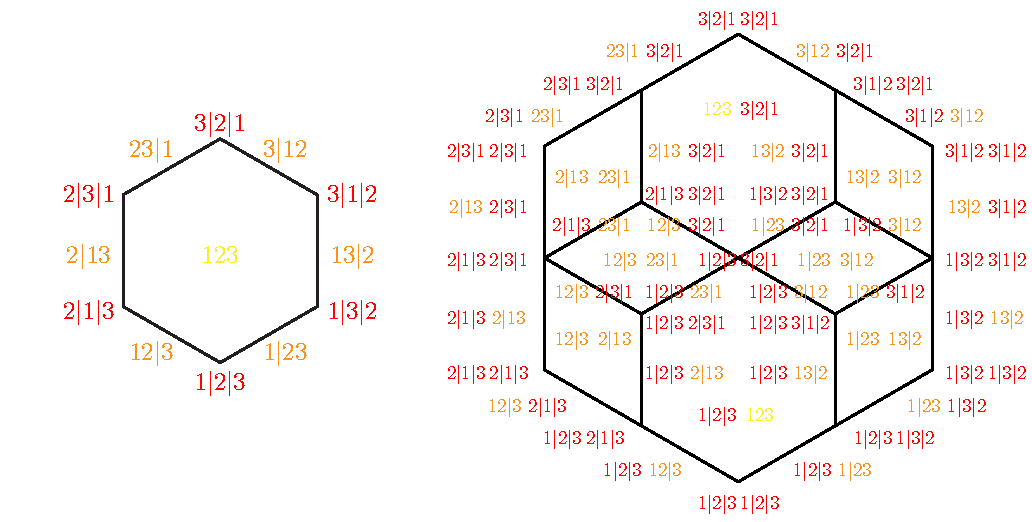
\includegraphics[scale=1.2]{diagonalPermutahedron2
}
		&
		\includegraphics[scale=1.2]{diagonalAssociahedron2}\hspace{1cm}
	\end{tabular}
}

\vspace{.1cm}

\large
Rencontre 3DMaps \\
Wednesday June 21st, 2023 \\
slides available at: \url{http://www.lix.polytechnique.fr/~pilaud/documents/presentations/diagonals.pdf}

\vspace*{-1cm}

\end{center}

%%%%%%%%%%

%\setul{0ex}{.3ex}
%\setstcolor{red}
%
%\begin{slide}{Unexpected talk}
%
%\vspace{.5cm}
%
%\phantom{\;\;{\red This}} \\[-.3cm]
%A usual talk consists in (?)
%
%\begin{itemize}
%
%\item a definition % {\red $\longleftarrow$ that we don't need for the talk}
%
%\item its motivation % \quad {\red $\longleftarrow$ I barely understand it ... see Daria's talk}
%
%\item some results that you hope the audience will remember \\ % {\red $\longleftarrow$ remember the message:} \\ 
%\phantom{.} % \hfill {\red ``diagonals have nice enumerative combinatorics''}
%
%\item no proofs (your time is limited) % \quad {\red $\longleftarrow$ this is the interesting part}
%
%\item concerning something you though about for years % \quad {\red $\longleftarrow$ I started in January}
%
%\item some pictures % \quad {\red $\longleftarrow$ \raisebox{-.3cm}{\scalebox{2}{\smiley{}}}}
%
%\item a joke % \quad {\red $\longleftarrow$ this slide is not the joke}
%
%\end{itemize}
%
%\end{slide}
%
%%%%
%
%\setul{0ex}{.3ex}
%\setstcolor{red}
%
%\begin{slide}{Unexpected talk}
%
%\vspace{.5cm}
%
%\;\;{\red This} \\[-.3cm]
%\st{A usual} talk consists in \st{(?)}
%
%\begin{itemize}
%
%\item a definition % {\red $\longleftarrow$ that we don't need for the talk}
%
%\item its motivation % \quad {\red $\longleftarrow$ I barely understand it ... see Daria's talk}
%
%\item some results that you hope the audience will remember \\ % {\red $\longleftarrow$ remember the message:} \\ 
%\phantom{.} % \hfill {\red ``diagonals have nice enumerative combinatorics''}
%
%\item no proofs (your time is limited) % \quad {\red $\longleftarrow$ this is the interesting part}
%
%\item concerning something you though about for years % \quad {\red $\longleftarrow$ I started in January}
%
%\item some pictures % \quad {\red $\longleftarrow$ \raisebox{-.3cm}{\scalebox{2}{\smiley{}}}}
%
%\item a joke % \quad {\red $\longleftarrow$ this slide is not the joke}
%
%\end{itemize}
%
%\end{slide}
%
%%%%
%
%\setul{0ex}{.3ex}
%\setstcolor{red}
%
%\begin{slide}{Unexpected talk}
%
%\vspace{.5cm}
%
%\;\;{\red This} \\[-.3cm]
%\st{A usual} talk consists in \st{(?)}
%
%\begin{itemize}
%
%\item a definition {\red $\longleftarrow$ that we don't need for the talk}
%
%\item its motivation % \quad {\red $\longleftarrow$ I barely understand it ... see Daria's talk}
%
%\item some results that you hope the audience will remember \\ % {\red $\longleftarrow$ remember the message:} \\ 
%\phantom{.} % \hfill {\red ``diagonals have nice enumerative combinatorics''}
%
%\item no proofs (your time is limited) % \quad {\red $\longleftarrow$ this is the interesting part}
%
%\item concerning something you though about for years % \quad {\red $\longleftarrow$ I started in January}
%
%\item some pictures % \quad {\red $\longleftarrow$ \raisebox{-.3cm}{\scalebox{2}{\smiley{}}}}
%
%\item a joke % \quad {\red $\longleftarrow$ this slide is not the joke}
%
%\end{itemize}
%
%\end{slide}
%
%%%%
%
%\setul{0ex}{.3ex}
%\setstcolor{red}
%
%\begin{slide}{Unexpected talk}
%
%\vspace{.5cm}
%
%\;\;{\red This} \\[-.3cm]
%\st{A usual} talk consists in \st{(?)}
%
%\begin{itemize}
%
%\item a definition {\red $\longleftarrow$ that we don't need for the talk}
%
%\item \st{its motivation} \quad {\red $\longleftarrow$ I barely understand it ... see Daria's talk}
%
%\item some results that you hope the audience will remember \\ % {\red $\longleftarrow$ remember the message:} \\ 
%\phantom{.} % \hfill {\red ``diagonals have nice enumerative combinatorics''}
%
%\item no proofs (your time is limited) % \quad {\red $\longleftarrow$ this is the interesting part}
%
%\item concerning something you though about for years % \quad {\red $\longleftarrow$ I started in January}
%
%\item some pictures % \quad {\red $\longleftarrow$ \raisebox{-.3cm}{\scalebox{2}{\smiley{}}}}
%
%\item a joke % \quad {\red $\longleftarrow$ this slide is not the joke}
%
%\end{itemize}
%
%\end{slide}
%
%%%%
%
%\setul{0ex}{.3ex}
%\setstcolor{red}
%
%\begin{slide}{Unexpected talk}
%
%\vspace{.5cm}
%
%\;\;{\red This} \\[-.3cm]
%\st{A usual} talk consists in \st{(?)}
%
%\begin{itemize}
%
%\item a definition {\red $\longleftarrow$ that we don't need for the talk}
%
%\item \st{its motivation} \quad {\red $\longleftarrow$ I barely understand it ... see Daria's talk}
%
%\item some results that \st{you hope the audience will remember} {\red $\longleftarrow$ remember the message:} \\ \phantom{.} \hfill {\red ``diagonals have nice enumerative combinatorics''}
%
%\item no proofs (your time is limited) % \quad {\red $\longleftarrow$ this is the interesting part}
%
%\item concerning something you though about for years % \quad {\red $\longleftarrow$ I started in January}
%
%\item some pictures % \quad {\red $\longleftarrow$ \raisebox{-.3cm}{\scalebox{2}{\smiley{}}}}
%
%\item a joke % \quad {\red $\longleftarrow$ this slide is not the joke}
%
%\end{itemize}
%
%\end{slide}
%
%%%%
%
%\setul{0ex}{.3ex}
%\setstcolor{red}
%
%\begin{slide}{Unexpected talk}
%
%\vspace{.5cm}
%
%\;\;{\red This} \\[-.3cm]
%\st{A usual} talk consists in \st{(?)}
%
%\begin{itemize}
%
%\item a definition {\red $\longleftarrow$ that we don't need for the talk}
%
%\item \st{its motivation} \quad {\red $\longleftarrow$ I barely understand it ... see Daria's talk}
%
%\item some results that \st{you hope the audience will remember} {\red $\longleftarrow$ remember the message:} \\ \phantom{.} \hfill {\red ``diagonals have nice enumerative combinatorics''}
%
%\item \st{no} proofs \st{(your time is limited)} \quad {\red $\longleftarrow$ this is the interesting part}
%
%\item concerning something you though about for years % \quad {\red $\longleftarrow$ I started in January}
%
%\item some pictures % \quad {\red $\longleftarrow$ \raisebox{-.3cm}{\scalebox{2}{\smiley{}}}}
%
%\item a joke % \quad {\red $\longleftarrow$ this slide is not the joke}
%
%\end{itemize}
%
%\end{slide}
%
%%%%
%
%\setul{0ex}{.3ex}
%\setstcolor{red}
%
%\begin{slide}{Unexpected talk}
%
%\vspace{.5cm}
%
%\;\;{\red This} \\[-.3cm]
%\st{A usual} talk consists in \st{(?)}
%
%\begin{itemize}
%
%\item a definition {\red $\longleftarrow$ that we don't need for the talk}
%
%\item \st{its motivation} \quad {\red $\longleftarrow$ I barely understand it ... see Daria's talk}
%
%\item some results that \st{you hope the audience will remember} {\red $\longleftarrow$ remember the message:} \\ \phantom{.} \hfill {\red ``diagonals have nice enumerative combinatorics''}
%
%\item \st{no} proofs \st{(your time is limited)} \quad {\red $\longleftarrow$ this is the interesting part}
%
%\item \st{concerning something you though about for years} \quad {\red $\longleftarrow$ I started in January}
%
%\item some pictures % \quad {\red $\longleftarrow$ \raisebox{-.3cm}{\scalebox{2}{\smiley{}}}}
%
%\item a joke % \quad {\red $\longleftarrow$ this slide is not the joke}
%
%\end{itemize}
%
%\end{slide}
%
%%%%
%
%\setul{0ex}{.3ex}
%\setstcolor{red}
%
%\begin{slide}{Unexpected talk}
%
%\vspace{.5cm}
%
%\;\;{\red This} \\[-.3cm]
%\st{A usual} talk consists in \st{(?)}
%
%\begin{itemize}
%
%\item a definition {\red $\longleftarrow$ that we don't need for the talk}
%
%\item \st{its motivation} \quad {\red $\longleftarrow$ I barely understand it ... see Daria's talk}
%
%\item some results that \st{you hope the audience will remember} {\red $\longleftarrow$ remember the message:} \\ \phantom{.} \hfill {\red ``diagonals have nice enumerative combinatorics''}
%
%\item \st{no} proofs \st{(your time is limited)} \quad {\red $\longleftarrow$ this is the interesting part}
%
%\item \st{concerning something you though about for years} \quad {\red $\longleftarrow$ I started in January}
%
%\item some pictures \quad {\red $\longleftarrow$ \raisebox{-.3cm}{\scalebox{2}{\smiley{}}}}
%
%\item a joke % \quad {\red $\longleftarrow$ this slide is not the joke}
%
%\end{itemize}
%
%\end{slide}
%
%%%%
%
%\setul{0ex}{.3ex}
%\setstcolor{red}
%
%\begin{slide}{Unexpected talk}
%
%\vspace{.5cm}
%
%\;\;{\red This} \\[-.3cm]
%\st{A usual} talk consists in \st{(?)}
%
%\begin{itemize}
%
%\item a definition {\red $\longleftarrow$ that we don't need for the talk}
%
%\item \st{its motivation} \quad {\red $\longleftarrow$ I barely understand it ... see Daria's talk}
%
%\item some results that \st{you hope the audience will remember} {\red $\longleftarrow$ remember the message:} \\ \phantom{.} \hfill {\red ``diagonals have nice enumerative combinatorics''}
%
%\item \st{no} proofs \st{(your time is limited)} \quad {\red $\longleftarrow$ this is the interesting part}
%
%\item \st{concerning something you though about for years} \quad {\red $\longleftarrow$ I started in January}
%
%\item some pictures \quad {\red $\longleftarrow$ \raisebox{-.3cm}{\scalebox{2}{\smiley{}}}}
%
%\item a joke \quad {\red $\longleftarrow$ this slide is not the joke}
%
%\end{itemize}
%
%\end{slide}

%%%%%%%%%%%%%%%%%%%%%%%%%%%%%%%%%%%%%%%%%%%%%%%%%%%%%%
%%%%%%%%%%%%%%%%%%%%%%%%%%%%%%%%%%%%%%%%%%%%%%%%%%%%%%

\partie{Diagonals of polytopes}

%%%%%%%%%%

\begin{slide}{Diagonals of polytopes}

$\poly{P}$ polytope in~$\R^d$

\vspace{-.5cm}
\emph{diagonal} of~$\poly{P} = \delta : \begin{array}[t]{ccc} \poly{P} & \to & \poly{P} \times \poly{P} \\ p & \mapsto & (p,p) \end{array}$
\hfill
\raisebox{-2cm}{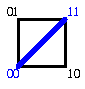
\includegraphics[scale=2.5]{diagonalSegment1}}

\vfill
\centerline{
\begin{tabular}{c@{}cc@{}c}
	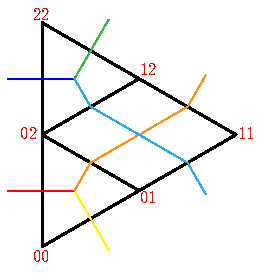
\includegraphics[scale=1.8]{diagonalTriangle3}
	&
	\phantom{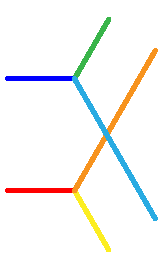
\includegraphics[scale=1.8]{diagonalTriangle4}}
	&
	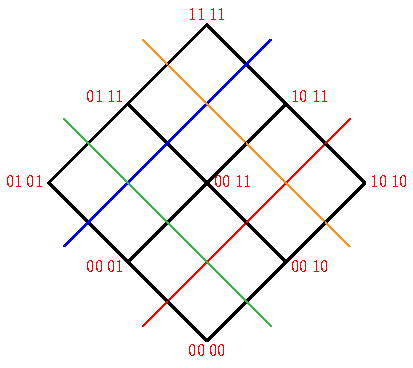
\includegraphics[scale=1.8]{diagonalSquarre3}
	\hspace{-1cm}
	&
	\phantom{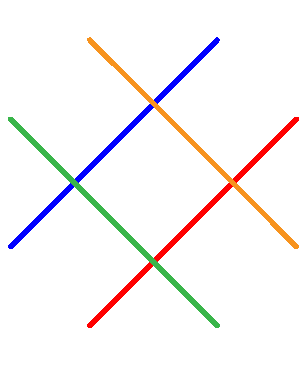
\includegraphics[scale=1.8]{diagonalSquarre4}}
	\\
	\multicolumn{2}{c}{\phantom{Alexander -- Whitney}}
	&
	\multicolumn{2}{c}{\phantom{Serre}}
	\\
	\multicolumn{2}{c}{\phantom{singular homology}}
	&
	\multicolumn{2}{c}{\phantom{cubical singular homology}}
\end{tabular}
}
\vspace{2.5cm}

\end{slide}

%%%

\begin{slide}{Diagonals of polytopes}

$\poly{P}$ polytope in~$\R^d$

\vspace{-.5cm}
\emph{diagonal} of~$\poly{P} = \delta : \begin{array}[t]{ccc} \poly{P} & \to & \poly{P} \times \poly{P} \\ p & \mapsto & (p,p) \end{array}$
\hfill
\raisebox{-2cm}{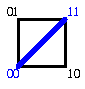
\includegraphics[scale=2.5]{diagonalSegment1}}

\vspace{.3cm}
\emph{cellular approximation} of the diagonal of~$\poly{P} =$ map $\poly{P} \to \poly{P} \times \poly{P}$ s.t.
\begin{compactitem}
\item its image is a union of faces of~$\poly{P} \times \poly{P}$
\item it agrees with~$\delta$ on the vertices of~$\poly{P}$
\item it is homotopic to~$\delta$
\end{compactitem}

\vspace{-4cm}
\hfill
\raisebox{2cm}{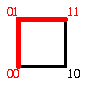
\includegraphics[scale=2.5]{diagonalSegment2}}

\vspace*{-10cm}

\vfill
\centerline{
\begin{tabular}{c@{}cc@{}c}
	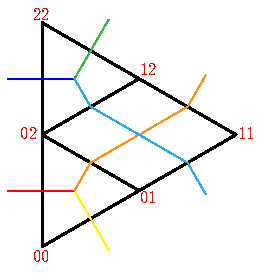
\includegraphics[scale=1.8]{diagonalTriangle3}
	&
	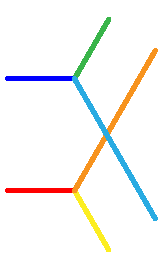
\includegraphics[scale=1.8]{diagonalTriangle4}
	&
	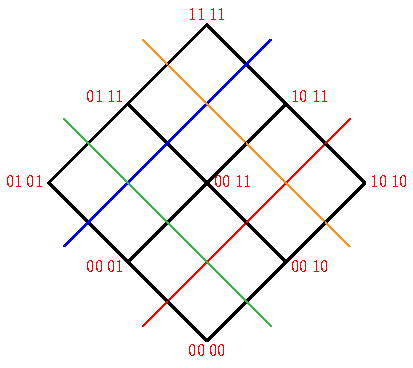
\includegraphics[scale=1.8]{diagonalSquarre3}
	\hspace{-1cm}
	&
	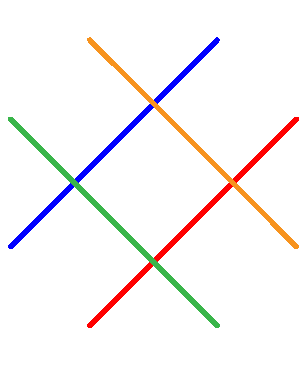
\includegraphics[scale=1.8]{diagonalSquarre4}
	\\
	\multicolumn{2}{c}{\phantom{Alexander -- Whitney}}
	&
	\multicolumn{2}{c}{\phantom{Serre}}
	\\
	\multicolumn{2}{c}{\phantom{singular homology}}
	&
	\multicolumn{2}{c}{\phantom{cubical singular homology}}
\end{tabular}
}
\vspace{2.5cm}

\end{slide}
%%%

\begin{slide}{Diagonals of polytopes}

$\poly{P}$ polytope in~$\R^d$

\vspace{-.5cm}
\emph{diagonal} of~$\poly{P} = \delta : \begin{array}[t]{ccc} \poly{P} & \to & \poly{P} \times \poly{P} \\ p & \mapsto & (p,p) \end{array}$
\hfill
\raisebox{-2cm}{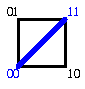
\includegraphics[scale=2.5]{diagonalSegment1}}

\vspace{.3cm}
\emph{cellular approximation} of the diagonal of~$\poly{P} =$ map $\poly{P} \to \poly{P} \times \poly{P}$ s.t.
\begin{compactitem}
\item its image is a union of faces of~$\poly{P} \times \poly{P}$
\item it agrees with~$\delta$ on the vertices of~$\poly{P}$
\item it is homotopic to~$\delta$
\end{compactitem}

\vspace{-4cm}
\hfill
\raisebox{2cm}{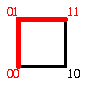
\includegraphics[scale=2.5]{diagonalSegment2}}

\vspace*{-10cm}

\vfill
\centerline{
\begin{tabular}{c@{}cc@{}c}
	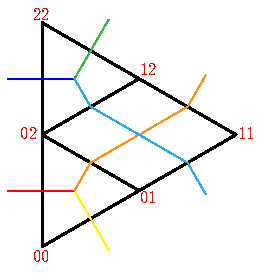
\includegraphics[scale=1.8]{diagonalTriangle3}
	&
	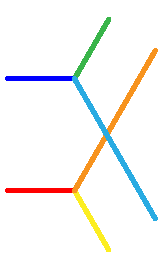
\includegraphics[scale=1.8]{diagonalTriangle4}
	&
	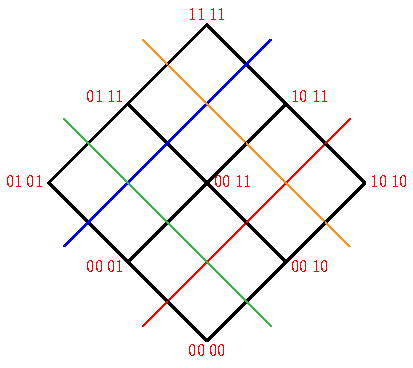
\includegraphics[scale=1.8]{diagonalSquarre3}
	\hspace{-1cm}
	&
	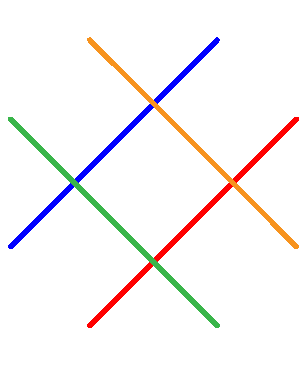
\includegraphics[scale=1.8]{diagonalSquarre4}
	\\
	\multicolumn{2}{c}{Alexander -- Whitney}
	&
	\multicolumn{2}{c}{Serre}
	\\
	\multicolumn{2}{c}{singular homology}
	&
	\multicolumn{2}{c}{cubical singular homology}
\end{tabular}
}
\vspace{2.5cm}

\end{slide}

%%%

\begin{slide}{Diagonals of polytopes}

\hfill\papier{Masuda -- Thomas -- Tonks -- Vallette '21}

\vspace{-.3cm}
\hfill\papier{Laplante-Anfossi '22} 

\vspace{-1.7cm}
any vertex of the fiber polytope \phantom{selected by~$(-v,v)$}
\[
\displaystyle
\sum \left( \!\! \begin{array}{ccc} \poly{P} \times \poly{P} & & (p,q) \\[.1cm] \rotatebox[origin=c]{-90}{$\xrightarrow{\hspace*{.6cm}}$} & , & \rotatebox[origin=c]{-90}{$\xmapsto{\hspace*{.6cm}}$} \\[.4cm] \poly{P} & & \frac{p+q}{2} \end{array} \!\! \right)
\]
gives a cellular approximation of the diagonal of~$\poly{P}$ \\
projecting back on~$\poly{P}$, we see it as a polyhedral subdivision of~$\poly{P}$
\vspace{-5cm}

\vfill
\hfill{\small \textcopyright\,G.\,Laplante-Anfossi} \\[-2.5cm]
\centerline{
\begin{tabular}{c@{}cc@{}c}
	\hspace{2cm}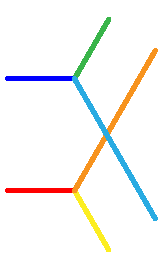
\includegraphics[scale=1.2]{diagonalTriangle4}
	&&
	\hspace{-1.3cm}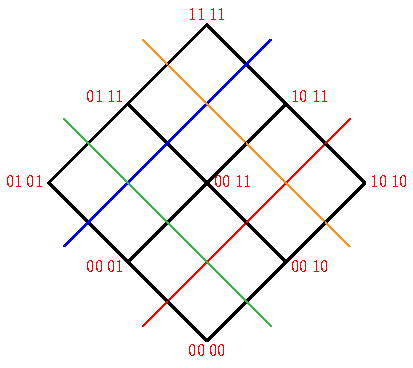
\includegraphics[scale=1.2]{diagonalSquarre3}\hspace{3.5cm}
	\\[-1.8cm]
	\raisebox{.9cm}{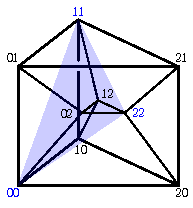
\includegraphics[scale=1.4]{diagonalTriangle1}}
	&
	\includegraphics[scale=.4]{diagonalSimplexGuillaume}
	&
	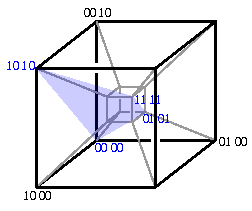
\includegraphics[scale=1.4]{diagonalSquarre1}
	&
	\includegraphics[scale=.45]{diagonalCubeGuillaume}
%	\\[-.5cm]
%	\multicolumn{2}{c}{$\displaystyle f_k(\Delta_{\Simplex(n)}) = (k+1) \binom{n+1}{k+2}$}
%	&
%	\multicolumn{2}{c}{$\displaystyle f_k(\Delta_{\Cube(n)}) = \binom{n}{k} 2^k 3^{n-k}$}
%	\\[.6cm]
%	\multicolumn{2}{c}{[OEIS, A127717]}
%	&
%	\multicolumn{2}{c}{[OEIS, A038220]}
\end{tabular}
}
\vspace{2cm}

\end{slide}

%%%

\begin{slide}{Diagonals of polytopes}

\hfill\papier{Masuda -- Thomas -- Tonks -- Vallette '21}

\vspace{-.3cm}
\hfill\papier{Laplante-Anfossi '22} 

\vspace{-1.7cm}
\parbox{\widthof{any}}{the\phantom{y}} vertex of the fiber polytope selected by~$(-v,v)$
\[
\displaystyle
\sum \left( \!\! \begin{array}{ccc} \poly{P} \times \poly{P} & & (p,q) \\[.1cm] \rotatebox[origin=c]{-90}{$\xrightarrow{\hspace*{.6cm}}$} & , & \rotatebox[origin=c]{-90}{$\xmapsto{\hspace*{.6cm}}$} \\[.4cm] \poly{P} & & \frac{p+q}{2} \end{array} \!\! \right)
\]
gives a cellular approximation of the diagonal of~$\poly{P}$ \\
projecting back on~$\poly{P}$, we see it as a polyhedral subdivision~$\Delta_{\poly{P},v}$ of~$\poly{P}$
\vspace{-5cm}

\vfill
\hfill{\small \textcopyright\,G.\,Laplante-Anfossi} \\[-2.5cm]
\centerline{
\begin{tabular}{c@{}cc@{}c}
	\hspace{2cm}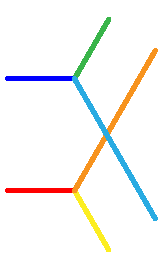
\includegraphics[scale=1.2]{diagonalTriangle4}
	&&
	\hspace{-1.3cm}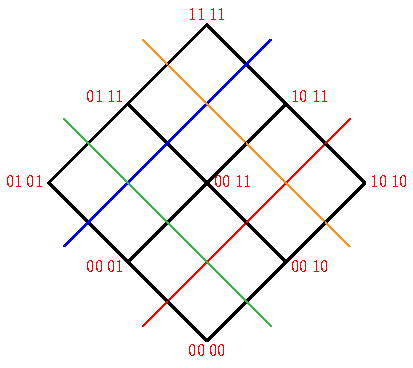
\includegraphics[scale=1.2]{diagonalSquarre3}\hspace{3.5cm}
	\\[-1.8cm]
	\raisebox{.9cm}{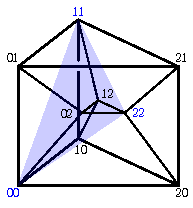
\includegraphics[scale=1.4]{diagonalTriangle1}}
	&
	\includegraphics[scale=.4]{diagonalSimplexGuillaume}
	&
	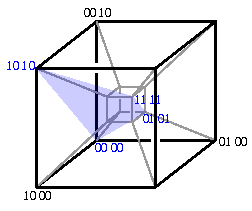
\includegraphics[scale=1.4]{diagonalSquarre1}
	&
	\includegraphics[scale=.45]{diagonalCubeGuillaume}
%	\\[-.5cm]
%	\multicolumn{2}{c}{$\displaystyle f_k(\Delta_{\Simplex(n)}) = (k+1) \binom{n+1}{k+2}$}
%	&
%	\multicolumn{2}{c}{$\displaystyle f_k(\Delta_{\Cube(n)}) = \binom{n}{k} 2^k 3^{n-k}$}
%	\\[.6cm]
%	\multicolumn{2}{c}{[OEIS, A127717]}
%	&
%	\multicolumn{2}{c}{[OEIS, A038220]}
\end{tabular}
}
\vspace{2cm}

\end{slide}

%%%

\begin{slide}{Diagonals of polytopes}

\theo{THM}{
\vspace{-1.2cm}
\begin{center}
combinatorics of the diagonal~$\Delta_{\poly{P},v}$ of~$\poly{P}$ \\
$\simeq$ \\
common refinement of two copies of the normal fan of~$\poly{P}$ translated by~$v$
\end{center}

\hfill\papier{Laplante-Anfossi '22} 

}

\vspace{1cm}
\centerline{
\begin{tabular}{c@{\hspace{-.5cm}}c@{\qquad}c@{\quad}c}
	\raisebox{.6cm}{\includegraphics[scale=1.4]{diagonalTriangle5}}
	&
	\raisebox{.6cm}{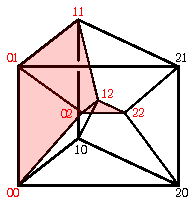
\includegraphics[scale=1.4]{diagonalTriangle2}}
	&
	\includegraphics[scale=1.2]{diagonalSquarre5}
	&
	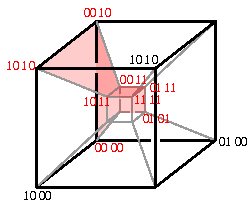
\includegraphics[scale=1.2]{diagonalSquarre2}
\end{tabular}
}

\end{slide}

%%%

\begin{slide}{Diagonals of polytopes}

\theo{THM}{
Faces of~$\Delta_{\poly{P},v} \subseteq$ pairs $(F,G)$ such that~$\max_v(F) \le \min_v(G)$

\hfill\papier{Laplante-Anfossi '22} 

}

\vspace{1cm}
When these are exactly the faces, it is called ``magical formula'' \\
This is the case for simplices, cubes, associahedra, but not permutahedra (see later)

\vspace{1cm}
\centerline{
\begin{tabular}{c@{\qquad}c}
	\raisebox{.6cm}{\includegraphics[scale=1.4]{diagonalTriangle6}}
	&
	\includegraphics[scale=1.2]{diagonalSquarre6}
	\\
	\phantom{$\displaystyle f_k(\Delta_{\Simplex(n)}) = (k+1) \binom{n+1}{k+2}$}
	&
	\phantom{$\displaystyle f_k(\Delta_{\Cube(n)}) = \binom{n}{k} 2^k 3^{n-k}$}
\end{tabular}
}

\end{slide}

%%%

\begin{slide}{Diagonals of polytopes}

\theo{THM}{
Faces of~$\Delta_{\poly{P},v} \subseteq$ pairs $(F,G)$ such that~$\max_v(F) \le \min_v(G)$

\hfill\papier{Laplante-Anfossi '22} 

}

\vspace{1cm}
When these are exactly the faces, it is called ``magical formula'' \\
This is the case for simplices, cubes, associahedra, but not permutahedra (see later)

\vspace{1cm}
\centerline{
\begin{tabular}{c@{\qquad}c}
	\raisebox{.6cm}{\includegraphics[scale=1.4]{diagonalTriangle6}}
	&
	\includegraphics[scale=1.2]{diagonalSquarre6}
	\\
	$\displaystyle f_k(\Delta_{\Simplex(n)}) = (k+1) \binom{n+1}{k+2}$
	% choose k+2 points of [n] where 2 consecutive are distinguished and might be equal, and the rest is distinct
	% this is the same as choosing k+2 points of [n+1], and the position of the consecutive pair of distinguished points among them
	% hence (k+1) \binom{n+1}{k+2}
	&
	$\displaystyle f_k(\Delta_{\Cube(n)}) = \binom{n}{k} 2^k 3^{n-k}$
	% choose a < b <= c < d in the boolean lattice such that |b-a| + |d-c| = k.
	% choose the positions of the ones in (b-a) + (d-c) => \binom{n}{k}
	% choose whether each of this ones is in (b-a) or in (d-c) => 2^k
	% choose the values of b and c on the remaining n-k positions to be either 00, 01 or 11 => 3^(n-k)
	\\[1cm]
	[OEIS, A127717]
	&
	[OEIS, A038220]
\end{tabular}
}

\end{slide}


%%%%%%%%%%%%%%%%%%%%%%%%%%%%%%%%%%%%%%%%%%%%%%%%%%%%%%
%%%%%%%%%%%%%%%%%%%%%%%%%%%%%%%%%%%%%%%%%%%%%%%%%%%%%%

\partie{Permutahedron \& associahedron}

%%%%%%%%%%

\begin{slide}{Lattices: Weak order \& Tamari lattice}

\vspace{.3cm}

\centerline{
	\begin{tabular}{l@{\qquad}l}
		\hspace{-1cm}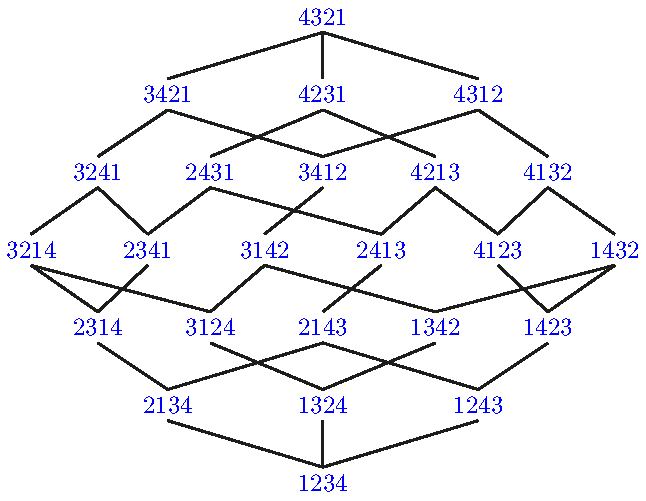
\includegraphics[scale=1.25]{weakOrder}
		&
		\includegraphics[scale=1]{TamariLattice}
		\\
		\emph{weak order} = permutations of~$[n]$
		&
		\emph{Tamari lattice} = binary trees on~$[n]$
		\\
		ordered by paths of simple transpositions
		&
		ordered by paths of right rotations
	\end{tabular}
}

\end{slide}

%%%

\begin{slide}{Lattices: Weak order \& Tamari lattice}

\vspace{.3cm}

\centerline{
	\begin{tabular}{l@{\qquad}l}
		\hspace{-1cm}\includegraphics[scale=1.25]{weakOrderZoom}
		&
		\includegraphics[scale=1]{TamariLatticeZoom1}\hspace{-1cm}
		\\
		\emph{weak order} = permutations of~$[n]$
		&
		\emph{Tamari lattice} = binary trees on~$[n]$
		\\
		ordered by paths of simple transpositions
		&
		ordered by paths of right rotations
	\end{tabular}
}

\end{slide}

%%%

\begin{slide}{Lattices: Weak order \& Tamari lattice}

\vspace{.3cm}

\centerline{
	\begin{tabular}{l@{\qquad}l}
		\hspace{-1cm}\includegraphics[scale=1.25]{sylvesterCongruence}
		&
		\includegraphics[scale=1]{TamariLattice}
		\\
		\emph{weak order} = permutations of~$[n]$
		&
		\emph{Tamari lattice} = binary trees on~$[n]$
		\\
		ordered by paths of simple transpositions
		&
		ordered by paths of right rotations
	\end{tabular}
}

\vspace{.6cm}
\emph{sylvester congruence} \begin{tabular}[t]{@{}l@{}} = equivalence classes are sets of linear extensions of binary trees \\ = equivalence classes are fibers of BST insertion \\ = rewriting rule~$UacVbW \equiv_{\mathrm{sylv}} UcaVbW$ with $a < b < c$\end{tabular}

\vspace{.6cm}
\emph{quotient lattice} = lattice on classes with $X \le Y  \iff  \exists \; x \in X, \; y \in Y, x \le y$

\end{slide}

%%%

\begin{slide}{Lattices: Weak order \& Tamari lattice}

\vspace{.3cm}

\centerline{
	\begin{tabular}{l@{\qquad}l}
		\hspace{-1cm}\includegraphics[scale=1.25]{sylvesterCongruenceZoom}
		&
		\includegraphics[scale=1]{TamariLatticeZoom2}\hspace{-3cm}
		\\
		\emph{weak order} = permutations of~$[n]$
		&
		\emph{Tamari lattice} = binary trees on~$[n]$
		\\
		ordered by paths of simple transpositions
		&
		ordered by paths of right rotations
	\end{tabular}
}

\vspace{.6cm}
\emph{sylvester congruence} \begin{tabular}[t]{@{}l@{}} = equivalence classes are sets of linear extensions of binary trees \\ = equivalence classes are fibers of BST insertion \\ = rewriting rule~$UacVbW \equiv_{\mathrm{sylv}} UcaVbW$ with $a < b < c$\end{tabular}

\vspace{.6cm}
\emph{quotient lattice} = lattice on classes with $X \le Y  \iff  \exists \; x \in X, \; y \in Y, x \le y$

\end{slide}

%%%%%%%%%%

\begin{slide}{Fans: braid fan \& sylvester fan}

\vspace{.6cm}

\centerline{
	\begin{tabular}{l@{\qquad}l}
		\includegraphics[scale=1.4]{braidFan}
		&
		\raisebox{-.6cm}{\includegraphics[scale=1.4]{sylvesterFan}}
		\\[-.5cm]
		\emph{braid fan} =
		&
		\emph{sylvester fan} = 
		\\
		$\quad \poly{C}(\sigma) = \set{\b{x} \in \R^n}{x_{\sigma(1)} \le \dots \le x_{\sigma(n)}}$
		&
		$\quad \poly{C}(T) = \set{\b{x} \in \R^n}{x_i \le x_j \text{ if $i \to j$ in $T$}}$
	\end{tabular}
}

\end{slide}

%%%

\begin{slide}{Fans: braid fan \& sylvester fan}

\vspace{.6cm}

\centerline{
	\begin{tabular}{l@{\qquad}l}
		\includegraphics[scale=1.4]{braidFanZoom}
		&
		\raisebox{-.6cm}{\includegraphics[scale=1.4]{sylvesterFanZoom}}
		\\[-.5cm]
		\emph{braid fan} =
		&
		\emph{sylvester fan} = 
		\\
		$\quad \poly{C}(\sigma) = \set{\b{x} \in \R^n}{x_{\sigma(1)} \le \dots \le x_{\sigma(n)}}$
		&
		$\quad \poly{C}(T) = \set{\b{x} \in \R^n}{x_i \le x_j \text{ if $i \to j$ in $T$}}$
	\end{tabular}
}

\end{slide}

%%%

\begin{slide}{Fans: braid fan \& sylvester fan}

\vspace{.6cm}

\centerline{
	\begin{tabular}{l@{\qquad}l}
		\includegraphics[scale=1.4]{braidFan}
		&
		\raisebox{-.6cm}{\includegraphics[scale=1.4]{sylvesterFan}}
		\\[-.5cm]
		\emph{braid fan} =
		&
		\emph{sylvester fan} = 
		\\
		$\quad \poly{C}(\sigma) = \set{\b{x} \in \R^n}{x_{\sigma(1)} \le \dots \le x_{\sigma(n)}}$
		&
		$\quad \poly{C}(T) = \set{\b{x} \in \R^n}{x_i \le x_j \text{ if $i \to j$ in $T$}}$
	\end{tabular}
}

\vspace{1cm}
\emph{quotient fan} = $\poly{C}(T)$ is obtained by glueing $\poly{C}(\sigma)$ for all linear extensions~$\sigma$ of~$T$

\end{slide}

%%%%%%%%%%

\begin{slide}{Polytopes: Permutahedron \& associahedron}

\vspace{.6cm}

\centerline{
	\begin{tabular}{ll}
		\includegraphics[scale=1.25]{permutahedron}
		&
		\raisebox{-.9cm}{\includegraphics[scale=1.25]{associahedron}}
		\\[.1cm]
		\emph{permutahedron} $\Perm(n)$
		&
		\emph{associahedron} $\Asso(n)$
		\\[.1cm]
		$\quad = \conv\bigset{[\sigma^{-1}(i)]_{i \in [n]}}{\sigma \in \fS_n}$
		&
		$\quad = \conv \set{[\ell(T,i) \cdot r(T,i)]_{i \in [n]}}{T \text{ binary tree}}$
		\\[.1cm]
		$\quad = \displaystyle \HH \, \cap \; \bigcap\nolimits_{\varnothing \ne J \subsetneq [n]} \HH_J$
		&
		$\quad = \displaystyle \HH \, \cap \; \bigcap\nolimits_{1 \le i < j \le n} \HH_{[i,j]}$
		\\[-.8cm]
		where $\HH_J = \bigset{\b{x} \in \R^{n}}{\sum_{j \in J} x_j \ge \binom{|J|+1}{2}}$ \hspace{-1cm}
		&
		\raisebox{.5cm}{\begin{minipage}{14cm}
		\flushright \papier{Stasheff ('63) \\ Shnider -- Sternberg ('93) \\[-.3cm] Loday ('04)}
		\end{minipage}}
	\end{tabular}
}
		
\end{slide}

%%%

\begin{slide}{Polytopes: Permutahedron \& associahedron}

\vspace{.6cm}

\centerline{
	\begin{tabular}{ll}
		\includegraphics[scale=1.25]{permutahedronZoom}
		&
		\raisebox{-.9cm}{\includegraphics[scale=1.25]{associahedronZoom}} \hspace*{-1cm}
		\\[.1cm]
		\emph{permutahedron} $\Perm(n)$
		&
		\emph{associahedron} $\Asso(n)$
		\\[.1cm]
		$\quad = \conv\bigset{[\sigma^{-1}(i)]_{i \in [n]}}{\sigma \in \fS_n}$
		&
		$\quad = \conv \set{[\ell(T,i) \cdot r(T,i)]_{i \in [n]}}{T \text{ binary tree}}$
		\\[.1cm]
		$\quad = \displaystyle \HH \, \cap \; \bigcap\nolimits_{\varnothing \ne J \subsetneq [n]} \HH_J$
		&
		$\quad = \displaystyle \HH \, \cap \; \bigcap\nolimits_{1 \le i < j \le n} \HH_{[i,j]}$
		\\[-.8cm]
		where $\HH_J = \bigset{\b{x} \in \R^{n}}{\sum_{j \in J} x_j \ge \binom{|J|+1}{2}}$ \hspace{-1cm}
		&
		\raisebox{.5cm}{\begin{minipage}{14cm}
		\flushright \papier{Stasheff ('63) \\ Shnider -- Sternberg ('93) \\[-.3cm] Loday ('04)}
		\end{minipage}}
	\end{tabular}
}
		
\end{slide}

%%%

\begin{slide}{Polytopes: Permutahedron \& associahedron}

\vspace{.6cm}

\centerline{
	\begin{tabular}{ll}
		\includegraphics[scale=1.25]{permutahedron}
		&
		\raisebox{-.9cm}{\includegraphics[scale=1.25]{associahedronPermutahedron}}
		\\[.1cm]
		\emph{permutahedron} $\Perm(n)$
		&
		\emph{associahedron} $\Asso(n)$
		\\[.1cm]
		$\quad = \conv\bigset{[\sigma^{-1}(i)]_{i \in [n]}}{\sigma \in \fS_n}$
		&
		$\quad = \conv \set{[\ell(T,i) \cdot r(T,i)]_{i \in [n]}}{T \text{ binary tree}}$
		\\[.1cm]
		$\quad = \displaystyle \HH \, \cap \; \bigcap\nolimits_{\varnothing \ne J \subsetneq [n]} \HH_J$
		&
		$\quad = \displaystyle \HH \, \cap \; \bigcap\nolimits_{1 \le i < j \le n} \HH_{[i,j]}$
		\\[-.8cm]
		where $\HH_J = \bigset{\b{x} \in \R^{n}}{\sum_{j \in J} x_j \ge \binom{|J|+1}{2}}$ \hspace{-1cm}
		&
		\raisebox{.5cm}{\begin{minipage}{14cm}
		\flushright \papier{Stasheff ('63) \\ Shnider -- Sternberg ('93) \\[-.3cm] Loday ('04)}
		\end{minipage}}
	\end{tabular}
}

%\gboite{
%	\emph{removahedron} = $\Asso(n)$ is obtained from $\Perm(n)$ by removing facet inequalities
%}
		
\end{slide}

%%%

\begin{slide}{Polytopes: Permutahedron \& associahedron}


\centerline{
\includemovie[autoplay, repeat, text={}, mouse=true]{600pt}{392pt}{polywood/outsidahedra_perm2asso2cube_penche_framed_fast_bothWays_cropped.mov}
}

\vfill
\includegraphics[scale=.5]{polywood/polywood}
\vspace{2.8cm}

\vspace{-.1cm}

\end{slide}

%%%%%%%%%%

\begin{slide}{lattices -- fans -- polytopes}

\vspace{.3cm}
\centerline{
	\begin{tabular}{l@{\hspace{2.4cm}}l}
		\emph{permutahedron} $\Perm(n)$
		&
		\emph{associahedron} $\Asso(n)$
		\\[.1cm]
		$\quad \Longrightarrow$ braid fan
		&
		$\quad \Longrightarrow$ Sylvester fan \hspace{2.9cm}
		\\[.1cm]
		$\quad \Longrightarrow$ weak order on permutations
		&
		$\quad \Longrightarrow$ Tamari lattice on binary trees \hspace{2.9cm}
		\\[.5cm]
		\includegraphics[scale=1.25]{permutahedronWeakOrder}
		&
		\raisebox{-.9cm}{\includegraphics[scale=1.25]{associahedronTamariLattice}}
		\\[-.8cm]
	\end{tabular}
}

\end{slide}

%%%%%%%%%%

\begin{slide}{$f$-vector of diagonals}

\centerline{
	\begin{tabular}{c@{}c}
		\hspace{2cm}\includegraphics[scale=1.15]{diagonalPermutahedron2}\hspace{2cm}
		&
		\hspace{2cm}\includegraphics[scale=1.15]{diagonalAssociahedron2}\hspace{2cm}
		\\[-.4cm]
		\includegraphics[scale=.45]{diagonalPermutahedronGuillaume}
		&
		\includegraphics[scale=.45]{diagonalAssociahedronGuillaume}
	\end{tabular}
}
\vspace{-10cm}

\hfill
\papier{Saneblidze -- Umble '04}

\vspace{-.3cm}
\hfill
\papier{Markl -- Shnider '06}

\vspace{-.3cm}
\hfill
\papier{Loday '11}

\vspace{6.8cm}
{\small \textcopyright\,G.\,Laplante-Anfossi}
\hfill
\papier{Masuda -- Thomas -- Tonks -- Vallette '21}

\vspace{-.3cm}
\hfill
\papier{Laplante-Anfossi '22} 

\end{slide}

%%%

\begin{slide}{$f$-vector of diagonals}

\centerline{
	\begin{tabular}{c@{}c}
		\hspace*{2cm}\includegraphics[scale=1.15]{diagonalPermutahedron2}\hspace{2cm}
		&
		\hspace{2cm}\includegraphics[scale=1.15]{diagonalAssociahedron2}\hspace*{2cm}
		\\[.5cm]
%		$\displaystyle f_k(\Delta_{\Perm(n)}) = \sum_{\b{F} \le \b{G}} \prod_{i \in [2]} \prod_{p \in G_i} (\# F_i[p]-1)!$
		$\displaystyle f_k = \sum_{\b{F} \le \b{G}} \prod_{i \in [2]} \prod_{p \in G_i} (\# F_i[p]-1)!$
		&
		$\displaystyle f_k = \frac{2}{(3n+1)(3n+2)} \binom{n-1}{k} \binom{4n+1-k}{n+1}$
		\\
%		$f_0(\Delta_{\Perm(n)}) = [x^n]  \; \exp \! \bigg( \sum_m \frac{x^m}{m(m+1)}\binom{2m}{m} \! \bigg)$
		$\displaystyle f_0 = [x^n]  \; \exp \! \bigg( \sum_m \frac{x^m}{m(m+1)}\binom{2m}{m} \! \bigg)$
		\\[1cm]
%		$f_{n-1}(\Delta_{\Perm(n)}) = 2 (n+1)^{n-2}$
		$f_{n-1} = 2 (n+1)^{n-2}$
		\\[-.8cm]
	\end{tabular}
}

\vspace{2.5cm}
\papier{Delcroix-Oger -- Josuat-Vergès -- Laplante-Anfossi -- P. -- Stoeckl '23$^+$}
\hfill
\papier{Bostan -- Chyzak -- P. '23$^+$}

\end{slide}

%%%%%%%%%%%%%%%%%%%%%%%%%%%%%%%%%%%%%%%%%%%%%%%%%%%%%%
%%%%%%%%%%%%%%%%%%%%%%%%%%%%%%%%%%%%%%%%%%%%%%%%%%%%%%

\partie{Diagonal of the associahedron}

\centerline{
	\raisebox{.5cm}{\includegraphics[scale=1.2]{diagonalAssociahedron1}}
	\includegraphics[scale=.6]{diagonalAssociahedronGuillaume}
}

\vspace{-2cm}
\hfill
{\small \textcopyright\,G.\,Laplante-Anfossi}

\begin{center}
\href{http://arxiv.org/abs/2303.10986}{\texttt{arXiv:2303.10986}}
\\[.1cm]
with \\
Alin BOSTAN (INRIA) \\
Frédéric CHYZAK (INRIA)
\end{center}

%%%%%%%%%%

\begin{slide}{Number of Tamari intervals}

$\Tam(n) = $ Tamari lattice on binary trees with $n$ nodes

\vfill
\centerline{\includegraphics[scale=1.1]{TamariLattices}}
\vspace{2.7cm}

\end{slide}

%%%

\begin{slide}{Number of Tamari intervals}

$\Tam(n) = $ Tamari lattice on binary trees with $n$ nodes

\vspace{.1cm}
\theo{THM}{
For any~$n \ge 1$, \hfill \papier{Chapoton '07}
\[
\# \{S \le T \in \Tam(n)\} = \frac{2}{(3n+1)(3n+2)} \binom{4n+1}{n+1}
\]

\vspace{-.4cm}
}

\vspace{.8cm}
$1, 3, 13, 68, 399, 2530, 16965, ...$ [OEIS A000260]
\vspace*{-1cm}

\vfill
\centerline{\includegraphics[scale=1.1]{TamariLattices}}
\vspace*{2.7cm}

\end{slide}

%%%%%%%%%%

\begin{slide}{First refined formula on Tamari intervals}

$\Tam(n) = $ Tamari lattice on binary trees with $n$ nodes \\
$\des(T) = $ number of binary trees {\red covered} by~$T$ \\
$\asc(T) = $ number of binary trees {\blue covering}~$T$

\vfill
\centerline{\includegraphics[scale=1.1]{TamariLatticesColored}}
\vspace{2.7cm}

\end{slide}

%%%

\begin{slide}{First refined formula on Tamari intervals}

$\Tam(n) = $ Tamari lattice on binary trees with $n$ nodes \\
$\des(T) = $ number of binary trees {\red covered} by~$T$ \\
$\asc(T) = $ number of binary trees {\blue covering}~$T$

\vspace{.5cm}
\theo{THM}{
For any~$n,k \ge 1$, \hfill \papier{Bostan -- Chyzak -- P. '23$^+$}
\[
\# \set{S \le T \in \Tam(n)}{\des(S) + \asc(T) = k} = \frac{2}{n(n+1)} \binom{n+1}{k+2} \binom{3n}{k}
\]

\vspace{-.4cm}
}

\vspace{1cm}
\centerline{\Large
	\begin{tabular}{c|ccccccccc|c}
		$n \backslash k$ & $0$ & $1$ & $2$ & $3$ & $4$ & $5$ & $6$ & $7$ & $8$ & $\Sigma$\\
		\hline
		$1$ & $1$ &&&&&&&&& $1$ \\
		$2$ & $1$ & $2$ &&&&&&&& $3$ \\
		$3$ & $1$ & $6$ & $6$ &&&&&&& $13$ \\
		$4$ & $1$ & $12$ & $33$ & $22$ &&&&&& $68$ \\
		$5$ & $1$ & $20$ & $105$ & $182$ & $91$ &&&&& $399$ \\
		$6$ & $1$ & $30$ & $255$ & $816$ & $1020$ & $408$ &&&& $2530$ \\
		$7$ & $1$ & $42$ & $525$ & $2660$ & $5985$ & $5814$ & $1938$ &&& $16965$ \\
		$8$ & $1$ & $56$ & $966$ & $7084$ & $24794$ & $42504$ & $33649$ & $9614$ && $118668$ \\
		$9$ & $1$ & $72$ & $1638$ & $16380$ & $81900$ & $215280$ & $296010$ & $197340$ & $49335$ & $857956$
	\end{tabular}
}

\end{slide}

%%%%%%%%%%

\begin{slide}{Canonical complex of the Tamari lattice}

$(L, \le, \meet, \join)$ lattice

\vspace{.3cm}
\emph{\parbox{\widthof{meet}}{\centering \red join} semidistributive}
\begin{tabular}[t]{@{}l}
$\iff$ $x \join y = x \join z$ implies $x \join (y \meet z) = x \join y$ for all~$x,y,z \in L$ \\
$\iff$ any~$x \in L$ admits a canonical \parbox{\widthof{meet}}{\centering \red join} representation \parbox{\widthof{$x = \bigMeet M$}}{\centering $x = \bigJoin \red J$}
\end{tabular}

\vspace{.3cm}
\emph{canonical \parbox{\widthof{meet}}{\centering \red join} complex}
\begin{tabular}[t]{@{}l}
$=$ simplicial complex of canonical \parbox{\widthof{meet}}{\centering \red join} representations \\
$=$ a simplex \parbox{\widthof{$M$}}{$\red J$\phantom{y}} for each element \parbox{\widthof{$\bigMeet M$}}{\centering $\bigJoin \red J$} of~$L$
\end{tabular}

\vspace{.2cm}
\centerline{
	\begin{overpic}[scale=1.7]{canonicalJoinComplexTamari3FullLetters}
		\put(98, 55){$\red \varnothing$}
		\put(30, 125){$\red a$}
		\put(170, 160){$\red b$}
		\put(30, 200){$\red c$}
		\put(83, 275){$\red a \join b$}
		\put(510, 100){$\red a$}
		\put(680, 100){$\red b$}
		\put(590, 70){$\red c$}
	\end{overpic}
}

\vspace*{-1.6cm}
\hfill\papier{Reading '15}

\vspace*{-.3cm}
\hfill\papier{Barnard '19}

\end{slide}

%%%

%\begin{slide}{Canonical complex of the Tamari lattice}
%
%$(L, \le, \meet, \join)$ lattice
%
%\vspace{.3cm}
%\emph{join semidistributive}
%\begin{tabular}[t]{@{}l}
%$\iff$ $x \join y = x \join z$ implies $x \join (y \meet z) = x \join y$ for all~$x,y,z \in L$ \\
%$\iff$ any~$x \in L$ admits a canonical join representation~$x = \bigJoin J$
%\end{tabular}
%
%\vspace{.3cm}
%\emph{canonical join complex} 
%\begin{tabular}[t]{@{}l}
%$=$ simplicial complex of canonical join representations \\
%$=$ a simplex~$J$ for each element~$\bigJoin J$ of~$L$
%\end{tabular}
%
%\vspace{.2cm}
%\centerline{\includegraphics[scale=1.7]{canonicalJoinComplexTamari3Full}}
%
%\vspace*{-1.6cm}
%\hfill\papier{Reading '15}
%
%\vspace*{-.3cm}
%\hfill\papier{Barnard '19}
%
%\end{slide}

%%%

\begin{slide}{Canonical complex of the Tamari lattice}

$(L, \le, \meet, \join)$ lattice

\vspace{.3cm}
\emph{{\blue meet} semidistributive}
\begin{tabular}[t]{@{}l}
$\iff$ $x \meet y = x \meet z$ implies $x \meet (y \join z) = x \meet y$ for all~$x,y,z \in L$ \\
$\iff$ any~$x \in L$ admits a canonical {\blue meet} representation~$x = \bigMeet \blue M$
\end{tabular}

\vspace{.3cm}
\emph{canonical {\blue meet} complex} 
\begin{tabular}[t]{@{}l}
$=$ simplicial complex of canonical {\blue meet} representations \\
$=$ a simplex~$\blue M$ for each element~$\bigMeet \blue M$ of~$L$
\end{tabular}

\vspace{.2cm}
\centerline{
	\begin{overpic}[scale=1.7]{canonicalJoinMeetComplexTamari3FullLetters}
		\put(98, 55){$\red \varnothing$}
		\put(30, 125){$\red a$}
		\put(170, 160){$\red b$}
		\put(30, 200){$\red c$}
		\put(83, 275){$\red a \join b$}
		\put(336, 55){$\blue b \meet c$}
		\put(280, 125){$\blue a$}
		\put(420, 160){$\blue b$}
		\put(280, 200){$\blue c$}
		\put(345, 275){$\blue \varnothing$}
		\put(510, 100){$\red a$}
		\put(680, 100){$\red b$}
		\put(590, 70){$\red c$}
		\put(590, 230){$\blue a$}
		\put(680, 200){$\blue b$}
		\put(510, 200){$\blue c$}
	\end{overpic}
}

\vspace*{-1.6cm}
\hfill\phantom{\papier{Reading '15}}

\vspace*{-.3cm}
\hfill
\papier{Albertin -- P. '22}

\end{slide}

%%%

\begin{slide}{Canonical complex of the Tamari lattice}

$(L, \le, \meet, \join)$ lattice

\vspace{.3cm}
\emph{semidistributive} 
\begin{tabular}[t]{@{}l}
$\iff$ join semidistributive and meet semidistributive \\
$\iff$ any~$x \in L$ admits canonical representations~$x = \bigJoin {\red J} = \bigMeet {\blue M}$
\end{tabular}

\vspace{.3cm}
\emph{canonical complex} 
\begin{tabular}[t]{@{}l}
$=$ simplicial complex of canonical representations \\
$=$ a simplex~${\red J} \sqcup {\blue M}$ for each interval~$\bigJoin {\red J} \le \bigMeet {\blue M}$ in~$L$
\end{tabular}

\vspace{.2cm}
\centerline{
	\begin{overpic}[scale=1.7]{canonicalComplexTamari3FullLetters}
		\put(98, 55){$\red \varnothing$}
		\put(30, 125){$\red a$}
		\put(170, 160){$\red b$}
		\put(30, 200){$\red c$}
		\put(83, 275){$\red a \join b$}
		\put(336, 55){$\blue b \meet c$}
		\put(280, 125){$\blue a$}
		\put(420, 160){$\blue b$}
		\put(280, 200){$\blue c$}
		\put(345, 275){$\blue \varnothing$}
		\put(510, 100){$\red a$}
		\put(680, 100){$\red b$}
		\put(590, 70){$\red c$}
		\put(590, 230){$\blue a$}
		\put(680, 200){$\blue b$}
		\put(510, 200){$\blue c$}
	\end{overpic}
}

\vspace*{-1.6cm}
\hfill\phantom{\papier{Reading '15}}

\vspace*{-.3cm}
\hfill\papier{Albertin -- P. '22}

\end{slide}

%%%

\begin{slide}{Canonical complex of the Tamari lattice}

$(L, \le, \meet, \join)$ lattice

\vspace{.3cm}
\emph{semidistributive} 
\begin{tabular}[t]{@{}l}
$\iff$ join semidistributive and meet semidistributive \\
$\iff$ any~$x \in L$ admits canonical representations~$x = \bigJoin {\red J} = \bigMeet {\blue M}$
\end{tabular}

\vspace{.3cm}
\emph{canonical complex} 
\begin{tabular}[t]{@{}l}
$=$ simplicial complex of canonical representations \\
$=$ a simplex~$J \sqcup M$ for each interval~$\bigJoin {\red J} \le \bigMeet {\blue M}$ in~$L$
\end{tabular}

\vspace{.2cm}
\centerline{\includegraphics[scale=1.7]{canonicalComplexTamari3Full}}

\vspace*{-1.6cm}
\hfill\papier{Reading '15}

\vspace*{-.3cm}
\hfill\papier{Albertin -- P. '22}

\end{slide}

%%%

\begin{slide}{Canonical complex of the Tamari lattice}

\vspace{.5cm}
\theo{THM}{
For any~$n,k \ge 1$, \hfill \papier{Bostan -- Chyzak -- P. '23$^+$}
\[
f_k(\mathbb{CC}_n) = \# \set{S \le T \in \Tam(n)}{\des(S) + \asc(T) = k} = \frac{2}{n(n+1)} \binom{n+1}{k+2} \binom{3n}{k}
\]

\vspace{-.4cm}
}

\vspace{1.15cm}
\centerline{\includegraphics[scale=1.7]{canonicalComplexTamari3Full}}

\vspace*{-1.6cm}
\hfill\papier{Reading '15}

\vspace*{-.3cm}
\hfill\papier{Albertin -- P. '22}

\end{slide}

%%%

\begin{slide}{Canonical complex of the Tamari lattice}

\vspace{.5cm}
\centerline{\includegraphics[scale=.95]{canonicalComplexTamari4}}

\centerline{$1 + 12 + 33 + 22 = 68$}

\vspace*{-1.45cm}
\hfill\papier{Reading '15}

\vspace*{-.3cm}
\hfill
\papier{Albertin -- P. '22}

\end{slide}

%%%%%%%%%%

\begin{slide}{Second refined formula on Tamari intervals}

$\Tam(n) = $ Tamari lattice on binary trees with $n$ nodes \\
$\des(T) = $ number of binary trees {\red covered} by~$T$ \\
$\asc(T) = $ number of binary trees {\blue covering}~$T$

\vspace{.5cm}
\theo{THM}{
For any~$n,k \ge 1$, \hfill \papier{Bostan -- Chyzak -- P. '23$^+$}
\[
%b_{n,k} \eqdef \sum_{\ell = k}^{n-1} a_{n,\ell} \binom{\ell}{k} = 
\sum_{S \le T \in \Tam(n)} \binom{\des(S) + \asc(T)}{k} = \frac{2}{(3n+1)(3n+2)} \binom{n-1}{k} \binom{4n+1-k}{n+1}
\]

\vspace{-.6cm}
}

\vspace{1cm}
\centerline{\Large
	\begin{tabular}{c|ccccccccc}
		$n \backslash k$ & $0$ & $1$ & $2$ & $3$ & $4$ & $5$ & $6$ & $7$ & $8$ \\
		\hline
		$1$ & $1$ \\
		$2$ & $3$ & $2$ \\
		$3$ & $13$ & $18$ & $6$ \\
		$4$ & $68$ & $144$ & $99$ & $22$ \\
		$5$ & $399$ & $1140$ & $1197$ & $546$ & $91$ \\
		$6$ & $2530$ & $9108$ & $12903$ & $8976$ & $3060$ & $408$ \\
		$7$ & $16965$ & $73710$ & $131625$ & $123500$ & $64125$ & $17442$ & $1938$ \\
		$8$ & $118668$ & $604128$ & $1302651$ & $1540770$ & $1078539$ & $446292$ & $100947$ & $9614$ \\
		$9$ & $857956$ & $5008608$ & $12660648$ & $18086640$ & $15958800$ & $8898240$ & $3058770$ & $592020$ & $49335$
	\end{tabular}
}

\end{slide}

%%%

\begin{slide}{Diagonal of the associahedron}

$\Delta_{\Asso(n)} = $ diagonal of $(n-1)$-dimensional associahedron

\centerline{\includegraphics[scale=1.3]{diagonalAssociahedron3}}

\end{slide}

%%%

\begin{slide}{Diagonal of the associahedron}

$\Delta_{\Asso(n)} = $ diagonal of $(n-1)$-dimensional associahedron

\centerline{\includegraphics[scale=1.3]{diagonalAssociahedron5}}

\end{slide}

%%%

\begin{slide}{Diagonal of the associahedron}

$\Delta_{\Asso(n)} = $ diagonal of $(n-1)$-dimensional associahedron

\centerline{\includegraphics[scale=1.3]{diagonalAssociahedron4}}

\theo{THM}{(Magical formula) \hfill\papier{Masuda -- Thomas -- Tonks -- Vallette '21}
\\[.3cm]
\centerline{$k$-faces of~$\Delta_{\Asso(n)}$ $\qquad \longleftrightarrow$ \begin{tabular}[t]{c} $(F,G)$ faces of $\Asso(n)$ with  \\ $\dim(F) + \dim(G) = k$ and $\max(F) \le \min(G)$ \end{tabular}}
}

\end{slide}

%%%

\begin{slide}{Diagonal of the associahedron}

$\Delta_{\Asso(n)} = $ diagonal of $(n-1)$-dimensional associahedron

\centerline{\includegraphics[scale=1.3]{diagonalAssociahedron4}}

\theo{THM}{
For any~$n,k \ge 1$, \hfill \papier{Bostan -- Chyzak -- P. '23$^+$}
\[
f_k(\Delta_{\Asso(n)}) = \!\!\! \sum_{S \le T \in \Tam(n)} \binom{\des(S) + \asc(T)}{k} = \frac{2}{(3n+1)(3n+2)} \binom{n-1}{k} \binom{4n+1-k}{n+1}
\]

\vspace{-.6cm}
}

\end{slide}

%%%%%%%%%%

\begin{slide}{Connection between the two formulas}

\vspace{.5cm}
\theo{THM}{
For any~$n,k \ge 1$, \hfill \papier{Bostan -- Chyzak -- P. '23$^+$}
\[
f_k(\mathbb{CC}_n) = \# \set{S \le T \in \Tam(n)}{\des(S) + \asc(T) = k} = \frac{2}{n(n+1)} \binom{n+1}{k+2} \binom{3n}{k}
\]

\vspace{-.4cm}
}

\vspace{.5cm}
\theo{THM}{
For any~$n,k \ge 1$, \hfill \papier{Bostan -- Chyzak -- P. '23$^+$}
\[
f_k(\Delta_{\Asso(n)}) = \!\!\! \sum_{S \le T \in \Tam(n)} \binom{\des(S) + \asc(T)}{k} = \frac{2}{(3n+1)(3n+2)} \binom{n-1}{k} \binom{4n+1-k}{n+1}
\]

\vspace{-.6cm}
}

\end{slide}

%%%%%%%%%%

\begin{slide}{Connection between the two formulas}

\vspace{.5cm}
\theo{THM}{
For any~$n,k \ge 1$, \hfill \papier{Bostan -- Chyzak -- P. '23$^+$}
\[
f_k(\mathbb{CC}_n) = \# \set{S \le T \in \Tam(n)}{\des(S) + \asc(T) = k} = \frac{2}{n(n+1)} \binom{n+1}{k+2} \binom{3n}{k}
\]

\vspace{-.4cm}
}

\vspace{.5cm}
\theo{THM}{
For any~$n,k \ge 1$, \hfill \papier{Bostan -- Chyzak -- P. '23$^+$}
\[
f_k(\Delta_{\Asso(n)}) = \!\!\! \sum_{S \le T \in \Tam(n)} \binom{\des(S) + \asc(T)}{k} = \frac{2}{(3n+1)(3n+2)} \binom{n-1}{k} \binom{4n+1-k}{n+1}
\]

\vspace{-.6cm}
}

\vspace{1cm}
Second formula follows from the first since ...

\theo{THM}{
For any~$n,k,r \in \N$, \hfill \papier{Bostan -- Chyzak -- P. '23$^+$}
\[
\sum_{\ell =k}^{n-1}  \binom{n+1}{\ell+2} \binom{r}{\ell} \binom{\ell}{k} = \frac{n(n+1)}{(r+1)(r+2)} \binom{n-1}{k} \binom{r+n+1-k}{n+1}.
\]

\vspace{-.6cm}
}

\vspace{.5cm}
... by application of Chu -- Vandermonde equality

\end{slide}

%%%%%%%%%%

\begin{slide}{Quadratic equation}

$n(T) = $ number of nodes of~$T$ \\
$\ell(T) =$ number of bounded edges on the left branch of~$T$

\[
\bbA(u,v,t,z) \eqdef \sum_{S \le T} u^{\ell(S)} v^{\ell(T)} t^{n(S)} z^{\des(S) + \asc(T)}
\]

\end{slide}

%%%

\begin{slide}{Quadratic equation}

$n(T) = $ number of nodes of~$T$ \\
$\ell(T) =$ number of bounded edges on the left branch of~$T$

\[
\bbA(u,v,t,z) \eqdef \sum_{S \le T} u^{\ell(S)} v^{\ell(T)} t^{n(S)} z^{\des(S) + \asc(T)}
\]

We want to compute

\[
A \eqdef A(t,z) \eqdef \sum_{S \le T} t^{n(S)} z^{\des(S) + \asc(T)} = \bbA(1,1,t,z)
\]

we will use $u$ and~$v$ as catalytic variables ...

\end{slide}

%%%

\begin{slide}{Quadratic equation}

$n(T) = $ number of nodes of~$T$ \\
$\ell(T) =$ number of bounded edges on the left branch of~$T$

\[
\bbA(u,v,t,z) \eqdef \sum_{S \le T} u^{\ell(S)} v^{\ell(T)} t^{n(S)} z^{\des(S) + \asc(T)}
\]

We want to compute

\[
A \eqdef A(t,z) \eqdef \sum_{S \le T} t^{n(S)} z^{\des(S) + \asc(T)} = \bbA(1,1,t,z)
\]

we will use $u$ and~$v$ as catalytic variables ...

\vspace{.5cm}
\theo{PROP}{
The generating functions~$A_u \eqdef \bbA(u,1,t,z)$ and~$A_1 \eqdef \bbA(1,1,t,z)$ satisfy the quadratic functional equation
\[
(u-1) A_u = t \big( u-1 + u (u+z-1) A_u - z A_1 \big) \big( 1 + uz A_u \big)
\]

\vspace{-.4cm}
}

\end{slide}

%%%%
%
%\begin{slide}{Quadratic equation}
%
%$n(T) = $ number of nodes of~$T$ \\
%$\ell(T) =$ number of bounded edges on the left branch of~$T$
%
%\[
%\bbA(u,v,t,z) \eqdef \sum_{S \le T} u^{\ell(S)} v^{\ell(T)} t^{n(S)} z^{\des(S) + \asc(T)}
%\]
%
%We want to compute
%
%\[
%A \eqdef A(t,z) \eqdef \sum_{S \le T} t^{n(S)} z^{\des(S) + \asc(T)} = \bbA(1,1,t,z)
%\]
%
%we will use $u$ and~$v$ as catalytic variables ...
%
%\vspace{1cm}
%Define
%\begin{alignat*}{4}
%A_u(t,z)
%& \eqdef \bbA(u,1,t,z) 
%& \text{and}\qquad &&
%A^\circ_u(t,z) & \eqdef \bbA(u,0,t,z) \\
%& = \sum_{S \le T} u^{\ell(S)} t^{n(S)} z^{\des(S) + \asc(T)}
%&&&
%& = \sum_{S \le T \text{ ind.}} u^{\ell(S)} t^{n(S)} z^{\des(S) + \asc(T)}
%\end{alignat*}
%
%\end{slide}
%
%%%%
%
%\begin{slide}{Quadratic equation}
%
%$n(T) = $ number of nodes of~$T$ \\
%$\ell(T) =$ number of bounded edges on the left branch of~$T$
%\[
%A_u(t,z) = \sum_{S \le T} u^{\ell(S)} t^{n(S)} z^{\des(S) + \asc(T)}
%\text{and}\qquad
%A^\circ_u(t,z) = \sum_{S \le T \text{ ind.}} u^{\ell(S)} t^{n(S)} z^{\des(S) + \asc(T)}
%\]
%
%\end{slide}
%
%%%%%%%%%%

\begin{slide}{Grafting decompositions}

\vspace{.5cm}
$S \backslash T = $ binary tree obtained by \emph{grafting}~$S$ on the leftmost leaf of~$T$ \\
$S = S_0 \backslash S_1 \backslash \dots \backslash S_k$ \emph{grafting decomposition}

\vspace{.5cm}
\centerline{\includegraphics[scale=1.8]{graftingDecompositionTree}}

\vspace{.5cm}
\theo{LEM}{
If~$S = S_0 \backslash S_1 \backslash \dots \backslash S_k$ and~$T = T_0 \backslash T_1 \backslash \dots \backslash T_k$ are s.t.~$n(S_i) = n(T_i)$ for all~$i \in [k]$, then \qquad\qquad\qquad $S \le T \iff S_i \le T_i$ for all~$i \in [k]$
\hfill \papier{Chapoton '07}
}

\vspace{.5cm}
\centerline{\includegraphics[scale=1.8]{graftingDecompositionInterval}}

\vspace{.3cm}
\theo{LEM}{
If~$S \le T$, then we can write~$S = S_0 \backslash S_1 \backslash \dots \backslash S_\ell$ and~$T = T_0 \backslash T_1 \backslash \dots \backslash T_\ell$ where \\ $\ell = \ell(T)$ and $n(S_i) = n(T_i)$ for all~$i \in [\ell]$
\hfill \papier{Chapoton '07}

}

\vspace{.5cm}
$\ell(T) =$ number of bounded edges on the left branch of~$T$

\end{slide}

%%%%%%%%%%

\begin{slide}{Quadratic equation}

$n(T) = $ number of nodes of~$T$ \\
$\ell(T) =$ number of bounded edges on the left branch of~$T$

\[
\bbA(u,v,t,z) \eqdef \sum_{S \le T} u^{\ell(S)} v^{\ell(T)} t^{n(S)} z^{\des(S) + \asc(T)}
\]

Consider
\begin{alignat*}{4}
A_u(t,z)
& \eqdef \bbA(u,1,t,z) 
& \qquad\text{and}\qquad &&
A^\circ_u(t,z) & \eqdef \bbA(u,0,t,z) \\
& = \text{all Tamari intervals}
&&&
& = \text{indecomposable intervals}
\end{alignat*}

\end{slide}

%%%

\begin{slide}{Quadratic equation}

$A_u = A_u(t,z) = \text{all Tamari intervals}$ \hfill $\displaystyle \sum_{S \le T} u^{\ell(S)} t^{n(S)} z^{\des(S) + \asc(T)}
$ \\[-.7cm]
$A^\circ_u = A^\circ_u(t,z) = \text{indecomposable intervals}$

\vfill
\hfill \papier{Chapoton '07}
\vspace*{2.5cm}

\end{slide}

%%%

\begin{slide}{Quadratic equation}

$A_u = A_u(t,z) = \text{all Tamari intervals}$ \hfill $\displaystyle \sum_{S \le T} u^{\ell(S)} t^{n(S)} z^{\des(S) + \asc(T)}
$ \\[-.7cm]
$A^\circ_u = A^\circ_u(t,z) = \text{indecomposable intervals}$

\vspace{.8cm}
1. 
$
\begin{array}[t]{ccccccccc}
\text{all intervals} & = & \text{indecomposable intervals} & \backslash & (&\varepsilon & + & \text{all intervals} &) \\ 
A_u & = & A^\circ_u && (&1 & + & u z A_u&)
\end{array}
$

\vfill
\hfill \papier{Chapoton '07}
\vspace*{2.5cm}

\end{slide}

%%%

\begin{slide}{Quadratic equation}

$A_u = A_u(t,z) = \text{all Tamari intervals}$ \hfill $\displaystyle \sum_{S \le T} u^{\ell(S)} t^{n(S)} z^{\des(S) + \asc(T)}
$ \\[-.7cm]
$A^\circ_u = A^\circ_u(t,z) = \text{indecomposable intervals}$

\vspace{.8cm}
1. 
$
\begin{array}[t]{ccccccccc}
\text{all intervals} & = & \text{indecomposable intervals} & \backslash & (&\varepsilon & + & \text{all intervals} &) \\ 
A_u & = & A^\circ_u && (&1 & + & u z A_u&)
\end{array}
$

\vspace{.8cm}
2. from any Tamari interval~$(S,T)$ where~$S = S_0 / S_1 / \dots / S_{\ell(S)}$, we can construct $\ell(S)+2$ indecomposable Tamari intervals~$(S_k',T')$ for~$0 \le k \le \ell(S)+1$, where
\[
S_k' = \big( S_0 / \dots / S_{k-1} \big) / Y \backslash \big( S_k / \dots / S_{\ell(S)} \big)
\qquad\text{and}\qquad
T' = Y \backslash T
\]

\begin{tabular}{c@{\quad}c@{\quad}c@{\quad}c}
	\includegraphics[scale=2]{proofGraftingDecompositions0} &
	\includegraphics[scale=2]{proofGraftingDecompositions1} &
	\includegraphics[scale=2]{proofGraftingDecompositions2} &
	\includegraphics[scale=2]{proofGraftingDecompositions3} \\
	$S_0' = Y / (S_0 / S_1 / S_2)$ &
	$S_1' = S_0 / Y \backslash (S_1 / S_2)$ &
	$S_2' = (S_0 / S_1) / Y \backslash S_2$ &
	$S_3' = (S_0 / S_1 / S_2) / Y$
\end{tabular}

\vspace{.5cm}
... and all indecomposable intervals are obtained this way

\[
A^\circ_u = t \Big( 1 + z \frac{u A_u - A_1}{u-1} + u A_u \Big)
\]

\vspace*{-3cm}

\vfill
\hfill \papier{Chapoton '07}
\vspace*{2.5cm}

\end{slide}

%%%

\begin{slide}{Quadratic equation}

$A_u = A_u(t,z) = \text{all Tamari intervals}$ \hfill $\displaystyle \sum_{S \le T} u^{\ell(S)} t^{n(S)} z^{\des(S) + \asc(T)}
$ \\[-.7cm]
$A^\circ_u = A^\circ_u(t,z) = \text{indecomposable intervals}$

\vspace{1cm}
1. \centerline{$A_u = A^\circ_u(1+u z A_u)$}

\vspace{1cm}
2. \centerline{$\displaystyle A^\circ_u = t \Big( 1 + z \frac{u A_u - A_1}{u-1} + u A_u \Big)$}

\vspace{.6cm}
\theo{PROP}{
The generating functions~$A_u \eqdef \bbA(u,1,t,z)$ and~$A_1 \eqdef \bbA(1,1,t,z)$ satisfy the quadratic functional equation
\[
(u-1) A_u = t \big( u-1 + u (u+z-1) A_u - z A_1 \big) \big( 1 + uz A_u \big)
\]

\vspace{-.4cm}
}

\vfill
\hfill \papier{Chapoton '07}
\vspace*{2.5cm}

\end{slide}

%%%%%%%%%%

\begin{slide}{Quadratic method}

\theo{PROP}{
The generating functions~$A_u \eqdef \bbA(u,1,t,z)$ and~$A_1 \eqdef \bbA(1,1,t,z)$ satisfy the quadratic functional equation
\[
(u-1) A_u = t \big( u-1 + u (u+z-1) A_u - z A_1 \big) \big( 1 + uz A_u \big)
\]

\vspace{-.4cm}
}

\vspace{.5cm}
Quadratic equation with a catalytic variable... \emph{quadratic method} \\
The discriminant of this quadratic polynomial must have multiple roots, hence, its own discriminant vanishes


\theo{CORO}{
The generating function~$A = A(t,z)$ is a root of the polynomial
\begin{gather*}
t^3 z^6 X^4 \\
{} + t^2 z^4 (t z^2 + 6 t z - 3 t + 3) X^3 \\
{} + t z^2 (6 t^2 z^3 + 9 t^2 z^2 - 12 t^2 z + 2 t z^2 + 3 t^2 - 6 t z + 21 t + 3) X^2 \\
{} + (12 t^3 z^4 - 4 t^3 z^3 - 9 t^3 z^2 - 10 t^2 z^3 + 6 t^3 z + 26 t^2 z^2  \hspace{3cm} \\ \hspace{6cm} - \; t^3 + 6 t^2 z + t z^2 + 3 t^2 - 12 t z - 3 t + 1) X \\
{} + t (8 t^2 z^3 - 12 t^2 z^2 + 6 t^2 z - t z^2 - t^2 + 10 t z + 2 t - 1)
\end{gather*}

\vspace{-.4cm}
}

\end{slide}

%%%%%%%%%%

\begin{slide}{Reparametrization}

\theo{CORO}{
The generating function~$A = A(t,z)$ is a root of the polynomial
\begin{gather*}
t^3 z^6 X^4 \\
{} + t^2 z^4 (t z^2 + 6 t z - 3 t + 3) X^3 \\
{} + t z^2 (6 t^2 z^3 + 9 t^2 z^2 - 12 t^2 z + 2 t z^2 + 3 t^2 - 6 t z + 21 t + 3) X^2 \\
{} + (12 t^3 z^4 - 4 t^3 z^3 - 9 t^3 z^2 - 10 t^2 z^3 + 6 t^3 z + 26 t^2 z^2  \hspace{3cm} \\ \hspace{6cm} - \; t^3 + 6 t^2 z + t z^2 + 3 t^2 - 12 t z - 3 t + 1) X \\
{} + t (8 t^2 z^3 - 12 t^2 z^2 + 6 t^2 z - t z^2 - t^2 + 10 t z + 2 t - 1)
\end{gather*}

\vspace{-.4cm}
}

\vspace{.5cm}
Reparametrize by
\[
t = \frac{s}{(s+1) (sz+1)^3} \qquad X = s - z s^2 - z s^3
\]

\theo{CORO}{
The generating function~$A = A(t,z)$ can be written
\[
A = S - z S^2 - z S^3
\qquad\text{where}\qquad
t = \frac{S}{(S+1) (Sz+1)^3}
\]

\vspace{-.4cm}
}


\end{slide}

%%%%%%%%%%

\begin{slide}{Lagrange inversion}

\theo{CORO}{
The generating function~$A = A(t,z)$ can be written
\[
A = S - z S^2 - z S^3
\qquad\text{where}\qquad
t = \frac{S}{(S+1) (Sz+1)^3}
\]

\vspace{-.4cm}
}

\theo{THM}{(Lagrange inversion)
If $S = t \psi(S)$, then
$\displaystyle [t^n] \; S^r = \frac{r}{n} \; [s^{n-r}] \; \phi(s)^n$
for any
$r \ge 1$

}

\vspace{1cm}
Here $\phi(s) \eqdef (s+1) (sz+1)^3$ \\
Hence $\displaystyle [s^a] \; \phi(s)^n = [s^a] (s+1)^n  (sz+1)^{3n} = \sum_{i+j=a} \binom{n}{i} \binom{3n}{j} z^j$ \\
Hence $\displaystyle [t^n z^k] S^r = \frac{r}{n} [s^{n-r} z^k] \phi(s)^n = \frac{r}{n} \binom{n}{n-r-k}  \binom{3n}{k} = \frac{r}{n} \binom{n}{k+r}  \binom{3n}{k}$ \\
Finally,
\[
[t^n z^k] A = [t^n z^k] S - [t^n z^{k-1}] S^2 - [t^n z^{k-1}] S^3 = \frac{2}{n(n+1)}  \binom{3n}{k}  \binom{n+1}{k+2}
\]

\end{slide}

%%%%%%%%%%

\begin{slide}{Bijections to planar triangulations}

$\Tam(n) = $ Tamari lattice on binary trees with $n$ nodes

\vspace{.1cm}
\theo{THM}{
For any~$n \ge 1$, \hfill \papier{Chapoton '07}
\[
\# \{S \le T \in \Tam(n)\} = \frac{2}{(3n+1)(3n+2)} \binom{4n+1}{n+1}
\]

\vspace{-.4cm}
}

\vspace{2cm}
Also counts rooted $3$-connected planar triangulations with $2n+2$ faces
\hfill\papier{Tutte}

\vspace{1cm}
\includegraphics[scale=3]{bijectionBinaryTrees}
\hfill\raisebox{2cm}{$\xleftrightarrow{\hspace*{9.35cm}}$}\hspace{-1cm}
\raisebox{-2cm}{\includegraphics[scale=3]{planarTriangulation}}

\end{slide}

%%%

\begin{slide}{Bijections to planar triangulations}

$\Tam(n) = $ Tamari lattice on binary trees with $n$ nodes

\vspace{.1cm}
\theo{THM}{
For any~$n \ge 1$, \hfill \papier{Chapoton '07}
\[
\# \{S \le T \in \Tam(n)\} = \frac{2}{(3n+1)(3n+2)} \binom{4n+1}{n+1}
\]

\vspace{-.4cm}
}

\vspace{2cm}
Also counts rooted $3$-connected planar triangulations with $2n+2$ faces
\hfill\papier{Tutte}

\vspace{1cm}
\includegraphics[scale=3]{bijectionBinaryTrees}
\hfill\raisebox{2cm}{$\xleftrightarrow{\hspace*{.7cm}}$}\hfill
\includegraphics[scale=3]{bijectionDyckPaths}
\hfill\raisebox{2cm}{$\xleftrightarrow{\hspace*{.7cm}}$}\hspace{-1cm}
\raisebox{-2cm}{\includegraphics[scale=3]{planarTriangulation}}

\end{slide}

%%%

\begin{slide}{Bijections to planar triangulations}

$\Tam(n) = $ Tamari lattice on binary trees with $n$ nodes

\vspace{.1cm}
\theo{THM}{
For any~$n \ge 1$, \hfill \papier{Chapoton '07}
\[
\# \{S \le T \in \Tam(n)\} = \frac{2}{(3n+1)(3n+2)} \binom{4n+1}{n+1}
\]

\vspace{-.4cm}
}

\vspace{2cm}
Also counts rooted $3$-connected planar triangulations with $2n+2$ faces
\hfill\papier{Tutte}

\vspace{1cm}
\includegraphics[scale=3]{bijectionBinaryTreesColored}
\hfill\raisebox{2cm}{$\xleftrightarrow{\hspace*{.7cm}}$}\hfill
\includegraphics[scale=3]{bijectionDyckPathsColored}
\hfill\raisebox{2cm}{$\xleftrightarrow{\hspace*{.7cm}}$}\hspace{-1cm}
\raisebox{-2cm}{\includegraphics[scale=3]{bijectionSchnyderWoods}}

\hfill\papier{Bernardi -- Bonichon, '09}

\end{slide}

%%%%%%%%%%

\begin{slide}{Schnyder woods}

\vspace{.5cm}
$M$ planar triangulation with external vertices~$v_0, v_1, v_3$ \\
$n$ internal nodes, $3n$ internal edges, $2n+1$ internal triangles \\[.5cm]
\emph{Schnyder wood} $=$ color (with~$0,1,2$) and orient the internal edges s.t.
\begin{compactitem}
\item the edges colored $i$ form a spanning tree oriented towards~$v_i$
\item each vertex satisfies the \emph{vertex rule}:
\end{compactitem}

\vspace{-4.5cm}
\hfill\includegraphics[scale=2]{SchnyderWoodsRule1}

\vspace{-1cm}
\phantom{Used for graph drawing and representations:}

\vspace{.3cm}
\centerline{\includegraphics[scale=.9]{boxicitySchnyderWood1}}

\vspace{-1cm}
\hfill\papier{Schnyder '89}

\end{slide}

%%%

\begin{slide}{Schnyder woods}

\vspace{.5cm}
$M$ planar triangulation with external vertices~$v_0, v_1, v_3$ \\
$n$ internal nodes, $3n$ internal edges, $2n+1$ internal triangles \\[.5cm]
\emph{Schnyder wood} $=$ color (with~$0,1,2$) and orient the internal edges s.t.
\begin{compactitem}
\item the edges colored $i$ form a spanning tree oriented towards~$v_i$
\item each vertex satisfies the \emph{vertex rule}:
\end{compactitem}

\vspace{-4.5cm}
\hfill\includegraphics[scale=2]{SchnyderWoodsRule1}

\vspace{-1cm}
Used for graph drawing and representations:

\vspace{.3cm}
\centerline{\includegraphics[scale=.9]{boxicitySchnyderWood2}}

\vspace{-1cm}
\hfill\papier{Schnyder '89}

\end{slide}

%%%

\begin{slide}{Schnyder woods}

\vspace{.5cm}
$M$ planar triangulation with external vertices~$v_0, v_1, v_3$ \\
$n$ internal nodes, $3n$ internal edges, $2n+1$ internal triangles \\[.5cm]
\emph{Schnyder wood} $=$ color (with~$0,1,2$) and orient the internal edges s.t.
\begin{compactitem}
\item the edges colored $i$ form a spanning tree oriented towards~$v_i$
\item each vertex satisfies the \emph{vertex rule}:
\end{compactitem}

\vspace{-4.5cm}
\hfill\includegraphics[scale=2]{SchnyderWoodsRule1}

\theo{THM}{
The Schnyder woods of a planar triangulation form a lattice structure under reorientations of clockwise essential cycles
}

\theo{CORO}{
Any planar triangulation admits a unique Schnyder wood with no clockwise~cycle

\vspace{-.1cm}
}

\vspace{1.5cm}
\hfill\papier{Ossona de Mendez '94}

\vspace{-.4cm}
\hfill\papier{Propp '97}
 
\vspace{-.4cm}
\hfill\papier{Felsner '04}

\end{slide}

%%%%%%%%%%

\begin{slide}{Bernardi -- Bonichon Bijection}

\vspace{.5cm}
\hspace{-1cm}
\begin{tabular}[t]{c}
	\includegraphics[scale=3]{bijectionBinaryTreesColored}
	\\[-.5cm]
	\includegraphics[scale=3]{bijectionDyckPathsColored}
	\\[-1cm]
	\includegraphics[scale=3]{bijectionSchnyderWoods}
\end{tabular}
\hspace{-1.5cm}
\raisebox{3cm}{
\begin{tabular}[t]{c}
	binary trees~$S \le T$
	\\
	with $n$ nodes
	\\[2.5cm]
	Dyck paths~$\mu \le \nu$
	\\
	with semilength~$n$
	\\[3cm]
	planar triangulations
	\\
	with $n$ internal vertices
\end{tabular}
}
\hspace{-.5cm}
\begin{tabular}[t]{l}
$\left\downarrow \begin{array}{rl} \text{contour of~$T$} \\ \text{transform} & \text{$\searrow$ to $\diagup$} \\ \text{and} & \text{$\nwarrow$ to $\diagdown$}\end{array} \right.$
\\[2.5cm]
$\left\uparrow \begin{array}{rl} \text{contour of~$\red T_0$} \\ \text{transform} & \text{${\red \leftarrow} \, \bullet$ to $\red \diagup$ and $\blue \diagup$} \\ & \text{${\red \rightarrow} \, \bullet$ to $\red \diagdown$}  \\ \text{and} & \text{${\blue \rightarrow} \, \bullet$ to $\blue \diagdown$} \end{array} \right.$
\end{tabular}

\vspace{1cm}
\hfill\papier{Bernardi -- Bonichon, '09}

\end{slide}

%%%

\begin{slide}{Bernardi -- Bonichon Bijection}

\vspace{.5cm}
\hspace{-1cm}
\begin{tabular}[t]{c}
	\includegraphics[scale=3]{bijectionAscentsDescents}
	\\[-.5cm]
	\includegraphics[scale=3]{bijectionValleysDoubleFalls}
	\\[-1cm]
	\includegraphics[scale=3]{bijectionSchnyderWoods}
\end{tabular}
\hspace{-1.5cm}
\raisebox{3cm}{
\begin{tabular}[t]{c@{\quad}c@{\quad}c}
	binary trees~$S \le T$
	&
	descents of~$S$
	&
	ascents of~$T$
	\\
	with $n$ nodes
	\\[2.5cm]
	Dyck paths~$\mu \le \nu$
	&
	double falls of~$\mu$
	&
	valleys of~$\nu$
	\\
	with semilength~$n$
	\\[3cm]
	planar triangulations
	&
	intermediate
	&
	intermediate
	\\
	with $n$ internal vertices
	&
	red vertices
	&
	blue vertices
\end{tabular}
}

\vspace{1cm}
\hfill\papier{Bernardi -- Bonichon, '09}

\end{slide}

%%%%%%%%%%

\begin{slide}{Counting internal degrees}

\includegraphics[scale=3]{bijectionAscentsDescents}
\hfill\raisebox{2cm}{$\xleftrightarrow{\hspace*{.7cm}}$}\hfill
\includegraphics[scale=3]{bijectionValleysDoubleFalls}
\hfill\raisebox{2cm}{$\xleftrightarrow{\hspace*{.7cm}}$}\hspace{-1cm}
\raisebox{-2cm}{\includegraphics[scale=3]{bijectionSchnyderWoods}}

%\vspace{-1.5cm}
%$f_{i,j,k} =$ \# Tamari intervals~$S \le T$ with
%\begin{tabular}[t]{@{}l}
%$\#\set{p}{\can(S)_p = \can(T)_p = {-}} = i$ \\
%$\#\set{p}{\can(S)_p = \can(T)_p = {+}} = j$ \\
%$\#\set{p}{\can(S)_p \ne  \can(T)_p} = k$ \\
%\end{tabular}

\theo{THM}{
%The generating function~$F \eqdef F(u,v,w) \eqdef \sum\limits_{i,j,k} f_{i,j,k} u^i v^j w^k$ is given by
The generating function~$\displaystyle F \eqdef F(u,v,w) \eqdef \sum_{S \le T} u^{\,\diagup\diagup} v^{\diagdown\diagdown\,} w^{\diagdown\,\,\diagup}$ is given by
\[
uvF = uU + vV + wUV - \frac{UV}{(1+U)(1+V)}
\]
where the series~$U \eqdef U(u,v,w)$ and~$V \eqdef V(u,v,w)$ satisfy the system
\begin{align*}
U & = (v+wU)(1+U)(1+V)^2 \\
V & = (u+wV)(1+V)(1+U)^2
\end{align*}

\vspace{-1.3cm}
\hfill\papier{Fusy -- Humbert '19}
}

\end{slide}

%%%

\begin{slide}{Counting internal degrees}

\includegraphics[scale=3]{bijectionAscentsDescents}
\hfill\raisebox{2cm}{$\xleftrightarrow{\hspace*{.7cm}}$}\hfill
\includegraphics[scale=3]{bijectionValleysDoubleFalls}
\hfill\raisebox{2cm}{$\xleftrightarrow{\hspace*{.7cm}}$}\hspace{-1cm}
\raisebox{-2cm}{\includegraphics[scale=3]{bijectionSchnyderWoods}}

%\vspace{-1.5cm}
%$f_{i,j,k} =$ \# Tamari intervals~$S \le T$ with
%\begin{tabular}[t]{@{}l}
%$\#\set{p}{\can(S)_p = \can(T)_p = {-}} = i$ \\
%$\#\set{p}{\can(S)_p = \can(T)_p = {+}} = j$ \\
%$\#\set{p}{\can(S)_p \ne  \can(T)_p} = k$ \\
%\end{tabular}

\theo{CORO}{
The function~$A \eqdef A(t,z) \eqdef \sum\limits_{S \le T} t^{n(S)} z^{\des(S) + \asc(T)} = tF(tz,tz,t)$ is given by
\[
t z^2 A = 2tz S + t S^2 - \frac{S^2}{(1+S)^2}
\]
where the series~$S \eqdef S(t,z)$ satisfies
\[
S = t(z+S)(1+S)^3
\]

\vspace{-.5cm}
}

\vspace{.8cm}
... and Lagrange inversion again
\hfill\papier{(thanks to Éric Fusy)}

\end{slide}

%%%%%%%%%%

\begin{slide}{Canopy}

\vspace{.5cm}
$T$ binary tree with~$n$ nodes, labeled in inorder and oriented towards its root. \\[.3cm]
\emph{canopy} of~$T =$ vector $\can(T) \in \{-,+\}^{n-1}$ with~$\can(T)_i = -$ \\
\begin{tabular}{@{\qquad$\iff$}l}
$(j+1)$st leaf of~$T$ is a right leaf \\
there is an oriented path joining its $j$th node to its $(j+1)$st node \\
the $j$th node of $T$ has an empty right subtree \\
the $(j+1)$st node of~$T$ has a non-empty left subtree \\
the cone corresponding to~$T$ is located in the halfspace~$x_j \le x_{j+1}$
\end{tabular}

\vspace{.5cm}
\centerline{\includegraphics[scale=3]{Canopy}}

\end{slide}

%%%

\begin{slide}{Canopy agreements}

\vspace{.5cm}
$T$ binary tree with~$n$ nodes, labeled in inorder and oriented towards its root. \\[.3cm]
\emph{canopy} of~$T =$ vector $\can(T) \in \{-,+\}^{n-1}$ with~$\can(T)_i = -$ \\
\begin{tabular}{@{\qquad$\iff$}l}
the $j$th node of $T$ has an empty right subtree \\
the $(j+1)$st node of~$T$ has a non-empty left subtree \\
\end{tabular}

\theo{LEM}{\qquad $\asc(T) = \#\set{i}{\can(T)_i = -}$ \quad and \quad $\des(T) = \#\set{i}{\can(T)_i = +}$}

\theo{LEM}{If~$S \le T$, then \\
\begin{tabular}{@{$\bullet$\;}l}
$\can(S) \le \can(T)$ componentwise \\
$\des(S) = \#\set{i}{\can(S)_i = \can(T)_i = +}$ and $\asc(S) = \#\set{i}{\can(S)_i = \can(T)_i = -}$
\end{tabular}
}

\theo{CORO}{
\hspace{2.5cm}
$\des(S) + \asc(T) = \#\text{canopy agreements between $S$ and $T$}$
}

\vspace{.5cm}
\centerline{
	\includegraphics[scale=3]{bijectionAscentsDescents}
	\qquad
	\includegraphics[scale=3]{bijectionCanopy}
}

\end{slide}

%%%%%%%%%%

\begin{slide}{Fang -- Fusy -- Nadeau bijection}

\vspace{.5cm}
\centerline{\includegraphics[scale=3]{bijectionRectangle1}}

\vfill
\hfill\papier{Fang -- Fusy -- Nadeau '23$^+$}
\vspace{3cm}

\end{slide}

%%%

\begin{slide}{Fang -- Fusy -- Nadeau bijection}

\vspace{.5cm}
\centerline{\includegraphics[scale=3]{bijectionRectangle2}}

\vfill
\hfill\papier{Fang -- Fusy -- Nadeau '23$^+$}
\vspace{3cm}

\end{slide}

%%%

\begin{slide}{Fang -- Fusy -- Nadeau bijection}

\vspace{.5cm}
\centerline{\includegraphics[scale=3]{bijectionRectangle3}}

\vfill
\hfill\papier{Fang -- Fusy -- Nadeau '23$^+$}
\vspace{3cm}

\end{slide}

%%%

\begin{slide}{Fang -- Fusy -- Nadeau bijection}

\vspace{.5cm}
\centerline{\includegraphics[scale=3]{bijectionRectangle4}}

\vfill
\hfill\papier{Fang -- Fusy -- Nadeau '23$^+$}
\vspace{3cm}

\end{slide}

%%%

\begin{slide}{Fang -- Fusy -- Nadeau bijection}

\vspace{.5cm}
\centerline{\includegraphics[scale=3]{bijectionRectangle5}}

\vfill
\hfill\papier{Fang -- Fusy -- Nadeau '23$^+$}
\vspace{3cm}

\end{slide}

%%%

\begin{slide}{Fang -- Fusy -- Nadeau bijection}

\vspace{.5cm}
\centerline{\includegraphics[scale=3]{bijectionRectangle6}}

\vfill
\hfill\papier{Fang -- Fusy -- Nadeau '23$^+$}
\vspace{3cm}

\end{slide}

%%%

\begin{slide}{Fang -- Fusy -- Nadeau bijection}

\vspace{.5cm}
\centerline{\includegraphics[scale=3]{bijectionRectangle7}}

\vfill
\hfill\papier{Fang -- Fusy -- Nadeau '23$^+$}
\vspace{3cm}

\end{slide}

%%%

\begin{slide}{Fang -- Fusy -- Nadeau bijection}

\vspace{.5cm}
\centerline{\includegraphics[scale=3]{bijectionRectangle8}}

\vfill
\hfill\papier{Fang -- Fusy -- Nadeau '23$^+$}
\vspace{3cm}

\end{slide}

%%%

\begin{slide}{Fang -- Fusy -- Nadeau bijection}

\vspace{-.8cm}
\[
\sum_{\text{meandres}} \phantom{(\; \teeM + \; \perpM + \; \crossM-1)} \; u \raisebox{.3cm}{\teeM} v \raisebox{.3cm}{\perpM} w \raisebox{.3cm}{\crossM} \; \phantom{= \sum_{\substack{\text{cyan} \\ \text{half-meanders}}} \!\!\!\!\!\! u \raisebox{.3cm}{\teeM} v \raisebox{.3cm}{\perpM} w \raisebox{.3cm}{\crossM} \cdot \sum_{\substack{\text{orange} \\ \text{half-meanders}}} \!\!\!\!\!\! u \raisebox{.3cm}{\teeM} v \raisebox{.3cm}{\perpM} w \raisebox{.3cm}{\crossM} }
\]

\vspace{.5cm}
\centerline{\includegraphics[scale=4]{bijectionRectangle9}}

\vfill
\hfill\papier{Fang -- Fusy -- Nadeau '23$^+$}
\vspace{3cm}

\end{slide}

%%%

\begin{slide}{Fang -- Fusy -- Nadeau bijection}

\vspace{-.8cm}
\[
\sum_{\text{meandres}} {(\; \teeM + \; \perpM + \; \crossM-1)} \; u \raisebox{.3cm}{\teeM} v \raisebox{.3cm}{\perpM} w \raisebox{.3cm}{\crossM} \; \phantom{= \sum_{\substack{\text{cyan} \\ \text{half-meanders}}} \!\!\!\!\!\! u \raisebox{.3cm}{\teeM} v \raisebox{.3cm}{\perpM} w \raisebox{.3cm}{\crossM} \cdot \sum_{\substack{\text{orange} \\ \text{half-meanders}}} \!\!\!\!\!\! u \raisebox{.3cm}{\teeM} v \raisebox{.3cm}{\perpM} w \raisebox{.3cm}{\crossM} }
\]

\vspace{.5cm}
\centerline{\includegraphics[scale=4]{bijectionRectangle10}}

\vfill
\hfill\papier{Fang -- Fusy -- Nadeau '23$^+$}
\vspace{3cm}

\end{slide}

%%%

\begin{slide}{Fang -- Fusy -- Nadeau bijection}

\vspace{-.8cm}
\[
\sum_{\text{meandres}} {(\; \teeM + \; \perpM + \; \crossM-1)} \; u \raisebox{.3cm}{\teeM} v \raisebox{.3cm}{\perpM} w \raisebox{.3cm}{\crossM} = \sum_{\substack{\text{cyan} \\ \text{half-meanders}}} \!\!\!\!\!\! u \raisebox{.3cm}{\teeM} v \raisebox{.3cm}{\perpM} w \raisebox{.3cm}{\crossM} \cdot \sum_{\substack{\text{orange} \\ \text{half-meanders}}} \!\!\!\!\!\! u \raisebox{.3cm}{\teeM} v \raisebox{.3cm}{\perpM} w \raisebox{.3cm}{\crossM} 
\]

\vspace{.5cm}
\centerline{\includegraphics[scale=4]{bijectionRectangle11}}

\vfill
\hfill\papier{Fang -- Fusy -- Nadeau '23$^+$}
\vspace{3cm}

\end{slide}

%%%

\begin{slide}{Fang -- Fusy -- Nadeau bijection}

\vspace{-.8cm}
\[
\sum_{\text{meandres}} {(\; \teeM + \; \perpM + \; \crossM-1)} \; u \raisebox{.3cm}{\teeM} v \raisebox{.3cm}{\perpM} w \raisebox{.3cm}{\crossM} = \quad\, \CHM(u,v,w) \; \cdot \; \OHM(u,v,w) \; \phantom{\sum_{\substack{\text{x} \\ \text{y}}}}
\]

\vspace{.55cm}
\centerline{\includegraphics[scale=4]{bijectionRectangle11}}

\vfill
\hfill\papier{Fang -- Fusy -- Nadeau '23$^+$}
\vspace{3cm}

\end{slide}

%%%

\begin{slide}{Fang -- Fusy -- Nadeau bijection}

\vspace{-.8cm}
\[
\sum_{\text{meandres}} {(\; \teeM + \; \perpM + \; \crossM-1)} \; u \raisebox{.3cm}{\teeM} v \raisebox{.3cm}{\perpM} w \raisebox{.3cm}{\crossM} = \quad\, \CHM(u,v,w) \; \cdot \; \OHM(u,v,w) \; \phantom{\sum_{\substack{\text{x} \\ \text{y}}}}
\]

\vspace{.55cm}
\centerline{\includegraphics[scale=4]{bijectionRectangle11}}

\[
\CHM = \frac{1}{(1-\CHM)^2} \Big( u + \frac{w \; \OHM}{1-\OHM} \Big)
\phantom{\qquad\text{and}\qquad
\OHM = \frac{1}{(1-\OHM)^2} \Big( v + \frac{w \; \CHM}{1-\CHM} \Big)}
\]

\vspace{.5cm}
\includegraphics[scale=4]{bijectionRectangle12}
\vspace{-3cm}

\vfill
\hfill\papier{Fang -- Fusy -- Nadeau '23$^+$}
\vspace{3cm}

\end{slide}

%%%

\begin{slide}{Fang -- Fusy -- Nadeau bijection}

\vspace{-.8cm}
\[
\sum_{\text{meandres}} {(\; \teeM + \; \perpM + \; \crossM-1)} \; u \raisebox{.3cm}{\teeM} v \raisebox{.3cm}{\perpM} w \raisebox{.3cm}{\crossM} = \quad\, \CHM(u,v,w) \; \cdot \; \OHM(u,v,w) \; \phantom{\sum_{\substack{\text{x} \\ \text{y}}}}
\]

\vspace{.55cm}
\centerline{\includegraphics[scale=4]{bijectionRectangle11}}

\[
\CHM = \frac{1}{(1-\CHM)^2} \Big( u + \frac{w \; \OHM}{1-\OHM} \Big)
\qquad\text{and}\qquad
\OHM = \frac{1}{(1-\OHM)^2} \Big( v + \frac{w \; \CHM}{1-\CHM} \Big)
\]

\vfill
\hfill\papier{Fang -- Fusy -- Nadeau '23$^+$}
\vspace{3cm}

\end{slide}

%%%

\begin{slide}{Fang -- Fusy -- Nadeau bijection}

\vspace{-.3cm}
\[
\sum_{\text{meandres}} {(\; \teeM + \; \perpM + \; \crossM-1)} \; (tz) \raisebox{.3cm}{\teeM} (tz) \raisebox{.3cm}{\perpM} t \raisebox{.3cm}{\crossM} = \HM(t,z)^2 \phantom{\sum_{\substack{\text{x} \\ \text{y}}}}
\]

\[
\text{where} \qquad \HM = \frac{t}{(1-\HM)^2} \Big( z + \frac{\HM}{1-\HM} \Big)
\]

\vfill
\hfill\papier{Fang -- Fusy -- Nadeau '23$^+$}
\vspace{3cm}

\end{slide}

%%%

\begin{slide}{Fang -- Fusy -- Nadeau bijection}

\vspace{-.3cm}
\[
\sum_{\text{meandres}} {(\; \teeM + \; \perpM + \; \crossM-1)} \; (tz) \raisebox{.3cm}{\teeM} (tz) \raisebox{.3cm}{\perpM} t \raisebox{.3cm}{\crossM} = \HM(t,z)^2 \phantom{\sum_{\substack{\text{x} \\ \text{y}}}}
\]

\[
\text{where} \qquad \HM = \frac{t}{(1-\HM)^2} \Big( z + \frac{\HM}{1-\HM} \Big)
\]

\vspace{1cm}
Lagrange inversion again:
\begin{align*}
[t^nz^k] \; \HM^2 
& = \frac{2}{n} \; [s^{n-2} z^k] \; \frac{1}{(1-s)^{2n}} \Big( z + \frac{s}{1-s} \Big)^n 
   = \frac{2}{n} \binom{n}{k} \; [s^{n-2}] \; \frac{s^{n-k}}{(1-s)^{3n-k}} \\
& = \frac{2}{n} \binom{n}{k} \; [s^{k-2}] \; \frac{1}{(1-s)^{3n-k}}
   = \frac{2}{n} \binom{n}{k} \binom{3n-3}{k-2}
\end{align*}

\vfill
\hfill\papier{Fang -- Fusy -- Nadeau '23$^+$}
\vspace{3cm}

\end{slide}

%%%

\begin{slide}{Fang -- Fusy -- Nadeau bijection}

\vspace{-.3cm}
\[
\sum_{\text{meandres}} {(\; \teeM + \; \perpM + \; \crossM-1)} \; (tz) \raisebox{.3cm}{\teeM} (tz) \raisebox{.3cm}{\perpM} t \raisebox{.3cm}{\crossM} = \HM(t,z)^2 \phantom{\sum_{\substack{\text{x} \\ \text{y}}}}
\]

\[
\text{where} \qquad \HM = \frac{t}{(1-\HM)^2} \Big( z + \frac{\HM}{1-\HM} \Big)
\]

\vspace{1cm}
Lagrange inversion again:
\begin{align*}
[t^nz^k] \; \HM^2 
& = \frac{2}{n} \; [s^{n-2} z^k] \; \frac{1}{(1-s)^{2n}} \Big( z + \frac{s}{1-s} \Big)^n 
   = \frac{2}{n} \binom{n}{k} \; [s^{n-2}] \; \frac{s^{n-k}}{(1-s)^{3n-k}} \\
& = \frac{2}{n} \binom{n}{k} \; [s^{k-2}] \; \frac{1}{(1-s)^{3n-k}}
   = \frac{2}{n} \binom{n}{k} \binom{3n-3}{k-2}
\end{align*}

\vspace{1cm}
Hence
\[
[t^n z^k] \; A(t,z) = \frac{1}{n+1} \; [t^{n+1} z^{k+2}] \; \HM^2 = \frac{2}{n(n+1)} \binom{n+1}{k+2} \binom{3n}{k}
\]

\vfill
\hfill\papier{Fang -- Fusy -- Nadeau '23$^+$}
\vspace{3cm}

\end{slide}

%%%%%%%%%%%%%%%%%%%%%%%%%%%%%%%%%%%%%%%%%%%%%%%%%%%%%%
%%%%%%%%%%%%%%%%%%%%%%%%%%%%%%%%%%%%%%%%%%%%%%%%%%%%%%

\partie{Diagonal of the permutahedron}

\centerline{
	\includegraphics[scale=1.2]{diagonalPermutahedron1}
	\qquad
	\includegraphics[scale=.5]{diagonalPermutahedronGuillaume}
}

\vspace{-2cm}
\hfill
{\small \textcopyright\,G.\,Laplante-Anfossi}

\vspace{.5cm}
\begin{center}
with \\
Bérénice DELCROIX-OGER (Univ.\,Montpellier) \\
Matthieu JOSUAT-VERGÈS (CNRS \& Univ.\,Paris Cité) \\
Guillaume LAPLANTE-ANFOSSI (Univ.\,Melbourne) \\
Kurt STOECKL (Univ.\,Melbourne)
\end{center}

%%%%%%%%%%

\begin{slide}{Diagonal of the permutahedron}

$\Delta_{\Perm(n)} = $ diagonal of $(n-1)$-dimensional permutahedron

\vspace{.2cm}
\centerline{\includegraphics[scale=1.3]{diagonalPermutahedron3}}

\vspace{-.2cm}
\theo{THM}{
$k$-faces of~$\Delta_{\Perm(n)}$ $\quad \longleftrightarrow$ \begin{tabular}[t]{c} $(\mu,\nu)$ ordered partitions of~$[n]$ such that \\ $\forall (I,J) \in D(n), \; \exists k \in [n], \; \# \mu_{[k]} \cap I > \# \mu_{[k]} \cap J$ \\ $\qquad\qquad\quad\; \text{ or } \exists \ell \in [n], \; \# \mu_{[\ell]} \cap I < \# \mu_{[\ell]} \cap J$ \end{tabular}

\vspace{-1cm}
\papier{Laplante-Anfossi '22} 

\vspace{.5cm}
where $D(n) \eqdef \{ (I,J) \ | \ I,J\subseteq [n], \, \#I = \#J, \, I \cap J = \varnothing, \min(I \cup J) \in I \}$

}

\end{slide}

%%%

\begin{slide}{Diagonal of the permutahedron}

$\Delta_{\Perm(n)} = $ diagonal of $(n-1)$-dimensional permutahedron

\vspace{.13cm}
\centerline{\includegraphics[scale=1.3]{diagonalPermutahedron4}}

\vspace{1cm}
\theo{PROP}{
$\BA[2][n] = $ two generically translated copies of the braid arrangement
\[
f_k \big( \, \Delta_{\Perm(n)} \, \big) = f_{n-k-1} \big( \, \BA[2][n] \, \big)
\]

\vspace{-.6cm}
\hfill\papier{Laplante-Anfossi '22} 

}

\end{slide}

%%%%%%%%%%

\begin{slide}{Flat poset \& Zaslavsky's theorem}

\emph{flat poset}~$\b{Fl}(\c{A})$ of an hyperplane arrangement~$\c{A} =$ \\
\hspace*{2cm}reverse inclusion poset on nonempty intersections of hyperplanes of~$\c{A}$

\vspace{.5cm}
\centerline{\includegraphics[scale=1.5]{intersectionPoset}}

\end{slide}

%%%

\begin{slide}{Flat poset \& Zaslavsky's theorem}

\emph{flat poset}~$\b{Fl}(\c{A})$ of an hyperplane arrangement~$\c{A} =$ \\
\hspace*{2cm}reverse inclusion poset on nonempty intersections of hyperplanes of~$\c{A}$

\vspace{.5cm}
\centerline{\includegraphics[scale=1.5]{intersectionPoset}}

\theo{EXM}{
\begin{tabular}[t]{@{}c@{\quad\;\;}c}
flat poset of braid arrangement~$\BA[][n]$ 
&
$\set{\b{x} \in \R^n}{\! \begin{array}{l} x_i = x_j \text{ for all } i,j \text{ in} \\ \text{the same part of } \pi \end{array} \! }$
\\
\rotatebox[origin=c]{90}{$\longleftrightarrow$}
&
\rotatebox[origin=c]{90}{$\longmapsto$}
\\[.3cm]
refinement poset on partitions of~$[n]$
&
$\pi$
\end{tabular}
\qquad

}

\end{slide}

%%%

\begin{slide}{Flat poset \& Zaslavsky's theorem}

\emph{flat poset}~$\b{Fl}(\c{A})$ of an hyperplane arrangement~$\c{A} =$ \\
\hspace*{2cm}reverse inclusion poset on nonempty intersections of hyperplanes of~$\c{A}$

\vspace{.5cm}
\centerline{\includegraphics[scale=1.5]{intersectionPoset}}

\vspace{.5cm}
\emph{M\"obius function} $\mu$ of a poset: $\mu(x,x) = 1$ and $\sum_{x \le y \le z} \mu(x,y) = 0$ for all~$x < z$

\end{slide}

%%%

\begin{slide}{Flat poset \& Zaslavsky's theorem}

\emph{flat poset}~$\b{Fl}(\c{A})$ of an hyperplane arrangement~$\c{A} =$ \\
\hspace*{2cm}reverse inclusion poset on nonempty intersections of hyperplanes of~$\c{A}$

\vspace{.5cm}
\centerline{
	\begin{overpic}[scale=1.5]{intersectionPoset}
		\put(453, -15){$1$}
		\put(310, 60){$-1$}
		\put(377, 60){$-1$}
		\put(444, 60){$-1$}
		\put(511, 60){$-1$}
		\put(578, 60){$-1$}
		\put(322, 195){$2$}
		\put(408, 195){$1$}
		\put(496, 195){$1$}
		\put(583, 195){$2$}
	\end{overpic}
}

\vspace{.5cm}
\emph{M\"obius function} $\mu$ of a poset: $\mu(x,x) = 1$ and $\sum_{x \le y \le z} \mu(x,y) = 0$ for all~$x < z$

\end{slide}

%%%

\begin{slide}{Flat poset \& Zaslavsky's theorem}

\emph{flat poset}~$\b{Fl}(\c{A})$ of an hyperplane arrangement~$\c{A} =$ \\
\hspace*{2cm}reverse inclusion poset on nonempty intersections of hyperplanes of~$\c{A}$

\vspace{.5cm}
\centerline{
	\begin{overpic}[scale=1.5]{intersectionPoset}
		\put(453, -15){$1$}
		\put(310, 60){$-1$}
		\put(377, 60){$-1$}
		\put(444, 60){$-1$}
		\put(511, 60){$-1$}
		\put(578, 60){$-1$}
		\put(322, 195){$2$}
		\put(408, 195){$1$}
		\put(496, 195){$1$}
		\put(583, 195){$2$}
	\end{overpic}
}

\vspace{.5cm}
\emph{M\"obius function} $\mu$ of a poset: $\mu(x,x) = 1$ and $\sum_{x \le y \le z} \mu(x,y) = 0$ for all~$x < z$

\vspace{.5cm}
\emph{M\"obius polynomial}
$\displaystyle \b{\mu}_{\c{A}}(x,y) = \sum_{F \le G} \mu(F,G) \, x^{\dim(F)} \, y^{\dim(G)}$

\theo{THM}{
$\b{f}_{\!\!\c{A}}(x) =  \b{\mu}_{\c{A}}(-x,-1)$
\qquad\text{and}\qquad
$\b{b}_\c{A}(x) =  \b{\mu}_{\c{A}}(-x,1)$
\hfill\papier{Zaslavsky '75}
}

\end{slide}

%%%%%%%%%%

\begin{slide}{$\ell$-braid arrangement \& partition forests}

\hspace{15cm}
\includegraphics[scale=1.5]{lBraidArrangement3}

\vspace{-11.5cm}
$\BA =$ 
\begin{tabular}[t]{@{}l}
union of $\ell$ \emph{generically} translated \\
copies of the braid arrangement
\end{tabular}

\end{slide}

%%%%%%%%%%

\begin{slide}{$\ell$-braid arrangement \& partition forests}

\hspace{15cm}
\includegraphics[scale=1.5]{lBraidArrangement3}

\vspace{-11.5cm}
$\BA =$ 
\begin{tabular}[t]{@{}l}
union of $\ell$ \emph{generically} translated \\
copies of the braid arrangement
\end{tabular}

\vspace{.5cm}
$(\ell,n)$ \emph{partition forest} $=$ \\
\hspace*{1cm}
\begin{tabular}[t]{@{}l}
$\ell$-tuple of partitions of~$[n]$ whose \\
intersection hypergraph is a forest
\end{tabular}

\includegraphics[scale=1.65]{partitionForest1}

\vfill
\theo{PROP}{
Intersection poset of~$\BA$ $\quad\longleftrightarrow\quad$ refinement poset on $(\ell,n)$ partition forests
}
\vspace{3cm}

\end{slide}

%%%%%%%%%%

\begin{slide}{$\ell$-braid arrangement \& partition forests}

\hspace{15cm}
\includegraphics[scale=1.5]{lBraidArrangement3}

\vspace{-11.5cm}
$\BA =$ 
\begin{tabular}[t]{@{}l}
union of $\ell$ \emph{generically} translated \\
copies of the braid arrangement
\end{tabular}

\vspace{.5cm}
$(\ell,n)$ \emph{partition forest} $=$ \\
\hspace*{1cm}
\begin{tabular}[t]{@{}l}
$\ell$-tuple of partitions of~$[n]$ whose \\
intersection hypergraph is a forest
\end{tabular}

\includegraphics[scale=1.65]{partitionForest2}

\vfill
\theo{PROP}{
Intersection poset of~$\BA$ $\quad\longleftrightarrow\quad$ refinement poset on $(\ell,n)$ partition forests
}
\vspace{3cm}

\end{slide}

%%%%%%%%%%

\begin{slide}{M\"obius polynomial}

$\P_p = $ refinement poset on partitions of~$[p]$ \\
$\PF = $ refinement poset on $(\ell,n)$ partition forests

\theo{FACT 1}{
The M\"obius function of~$\P_p$ is
$
\displaystyle
\mu(\hat 0, \hat 1) = (-1)^{p-1} (p-1)!
$
}

\theo{FACT 2}{
In~$\P_p$,
\qquad\quad
$
\displaystyle
[F,G] \simeq \prod_{p \in G} \P_{\# F[p]}
$
\qquad\quad
where~$F[p] =$ restriction of~$F$ to~$p$
}

\theo{FACT 2}{
$
\displaystyle
[\b{F}, \b{G}] \simeq \prod_{i \in [\ell]} [F_i, G_i]
$
\qquad
for~$\b{F} = (F_1, \dots, F_\ell)$ and~$\b{G} = (G_1, \dots, G_\ell)$ in~$\PF$
}

\theo{FACT 4}{
M\"obius is multiplicative
\qquad
\(
\mu_{P \times Q} \big( (p,q), (p’,q’) \big) = \mu_P(p,p’) \cdot \mu_Q(q,q’)
\)

}

%\theo{THM}{
%\hspace*{5.5cm}
%$
%\displaystyle
%f_{n-k-1}(\BA) = \sum_{\b{F} \le \b{G}} \prod_{i \in [\ell]} \prod_{p \in G_i} (\# F_i[p]-1)!
%$
%\\
%where~$\b{F} \le \b{G}$ are intervals of~$\PF$ such that~$\sum_{i \in [\ell]} \#F_i = \ell n - k$
%
%\vspace{.2cm}
%\hfill\papier{Delcroix-Oger -- Josuat-Vergès -- Laplante-Anfossi -- P. -- Stoeckl '23$^+$}
%\vspace{-.2cm}
%
%}

\end{slide}

%%%

\begin{slide}{M\"obius polynomial}

$\P_p = $ refinement poset on partitions of~$[p]$ \\
$\PF = $ refinement poset on $(\ell,n)$ partition forests

\theo{FACT 1}{
The M\"obius function of~$\P_p$ is
$
\displaystyle
\mu(\hat 0, \hat 1) = (-1)^{p-1} (p-1)!
$
}

\theo{FACT 2}{
In~$\P_p$,
\qquad\quad
$
\displaystyle
[F,G] \simeq \prod_{p \in G} \P_{\# F[p]}
$
\qquad\quad
where~$F[p] =$ restriction of~$F$ to~$p$
}

\theo{FACT 2}{
$
\displaystyle
[\b{F}, \b{G}] \simeq \prod_{i \in [\ell]} [F_i, G_i]
$
\qquad
for~$\b{F} = (F_1, \dots, F_\ell)$ and~$\b{G} = (G_1, \dots, G_\ell)$ in~$\PF$
}

\theo{FACT 4}{
M\"obius is multiplicative
\qquad
\(
\mu_{P \times Q} \big( (p,q), (p’,q’) \big) = \mu_P(p,p’) \cdot \mu_Q(q,q’)
\)

}

\theo{THM}{
$
\qquad
\displaystyle
\b{\mu}_{\BA} = x^{n-1-\ell n} y^{n-1-\ell n} \sum_{\b{F} \le \b{G}} \prod_{i \in [\ell]} x^{\#F_i} y^{\#G_i} \prod_{p \in G_i} (-1)^{\#F_i[p]-1} (\# F_i[p]-1)!
$

\vspace{.5cm}
\hfill\papier{Delcroix-Oger -- Josuat-Vergès -- Laplante-Anfossi -- P. -- Stoeckl '23$^+$}
\vspace{-.2cm}

}

\end{slide}

%%%%%%%%%%

\begin{slide}{face polynomial}

\theo{THM}{
\hspace*{4.5cm}
$
\displaystyle
\b{f}_{\!\BA}(x) = x^{n-1-\ell n}\sum_{\b{F} \le \b{G}} \prod_{i \in [\ell]} x^{\#F_i} \prod_{p \in G_i} (\# F_i[p]-1)!
$

\vspace{.5cm}
\hfill\papier{Delcroix-Oger -- Josuat-Vergès -- Laplante-Anfossi -- P. -- Stoeckl '23$^+$}
\vspace{-.2cm}

}

\vfill
\centerline{
	\begin{tabular}{c@{\hspace{.7cm}}c@{\hspace{.7cm}}c}
		\includegraphics[scale=1]{lBraidArrangement1}
		&
		\includegraphics[scale=1]{lBraidArrangement2}
		&
		\includegraphics[scale=1]{lBraidArrangement3}		
		\\
		\begin{tabular}[t]{c|cccc|c}
			$n \backslash k$ & $0$ & $1$ & $2$ & $3$ & $\Sigma$ \\
			\hline
			$1$ & $1$ &&&& $1$ \\
			$2$ & $2$ & $1$ &&& $3$ \\
			$3$ & $6$ & $6$ & $1$ && $13$ \\
			$4$ & $24$ & $36$ & $14$ & $1$ & $75$ \\
		\end{tabular}
		&
		\begin{tabular}[t]{c|cccc|c}
			$n \backslash k$ & $0$ & $1$ & $2$ & $3$ & $\Sigma$ \\
			\hline
			$1$ & $1$ &&&& $1$ \\
			$2$ & $3$ & $2$ &&& $5$ \\
			$3$ & $17$ & $24$ & $8$ && $49$ \\
			$4$ & $149$ & $324$ & $226$ & $50$ & $749$
		\end{tabular}
		&
		\begin{tabular}[t]{c|cccc|c}
			$n \backslash k$ & $0$ & $1$ & $2$ & $3$ & $\Sigma$ \\
			\hline
			$1$ & $1$ &&&& $1$ \\
			$2$ & $4$ & $3$ &&& $7$ \\
			$3$ & $34$ & $54$ & $21$ && $109$ \\
			$4$ & $472$ & $1152$ & $924$ & $243$ & $2791$
		\end{tabular}
%		&
%		\begin{tabular}[t]{c|cccc|c}
%			$n \backslash k$ & $0$ & $1$ & $2$ & $3$ & $\Sigma$ \\
%			\hline
%			$1$ & $1$ &&&& $1$ \\
%			$2$ & $5$ & $4$ &&& $9$ \\
%			$3$ & $57$ & $96$ & $40$ && $193$ \\
%			$4$ & $1089$ & $2808$ & $2396$ & $676$ & $6969$
%		\end{tabular}
		\\
		\hspace{8.5cm} & \hspace{8.5cm} & \hspace{9.5cm}
		\\[-.8cm]
		$\ell = 1$ & $\ell = 2$ & $\ell = 3$ % & $\ell = 4$
	\end{tabular}
}
\vspace*{2.5cm}

\end{slide}

%%%%%%%%%%

\begin{slide}{bounded face polynomial}

\theo{THM}{
\hspace*{3.5cm}
$
\displaystyle
\b{b}_{\BA}(x) = (-1)^\ell x^{n-1-\ell n} \sum_{\b{F} \le \b{G}} \prod_{i \in [\ell]} x^{\#F_i} \prod_{p \in G_i} -(\# F_i[p]-1)!
$

\vspace{.4cm}
\hfill\papier{Delcroix-Oger -- Josuat-Vergès -- Laplante-Anfossi -- P. -- Stoeckl '23$^+$}
\vspace{-.2cm}

}

\vfill
\centerline{
	\begin{tabular}{c@{\hspace{.7cm}}c@{\hspace{.7cm}}c}
		\includegraphics[scale=.9]{lBraidArrangement1}
		&
		\includegraphics[scale=.9]{lBraidArrangement2}
		&
		\includegraphics[scale=.9]{lBraidArrangement3}		
		\\
		\begin{tabular}[t]{c|cccc|c}
			$n \backslash k$ & $0$ & $1$ & $2$ & $3$ & $\Sigma$ \\
			\hline
			$1$ & $1$ &&&& $1$ \\
			$2$ & $0$ & $1$ &&& $1$ \\
			$3$ & $0$ & $0$ & $1$ && $1$ \\
			$4$ & $0$ & $0$ & $0$ & $1$ & $1$
		\end{tabular}
		&
		\begin{tabular}[t]{c|cccc|c}
			$n \backslash k$ & $0$ & $1$ & $2$ & $3$ & $\Sigma$ \\
			\hline
			$1$ & $1$ &&&& $1$ \\
			$2$ & $1$ & $2$ &&& $3$ \\
			$3$ & $5$ & $12$ & $8$ && $25$ \\
			$4$ & $43$ & $132$ & $138$ & $50$ & $363$
		\end{tabular}
		&
		\begin{tabular}[t]{c|cccc|c}
			$n \backslash k$ & $0$ & $1$ & $2$ & $3$ & $\Sigma$ \\
			\hline
			$1$ & $1$ &&&& $1$ \\
			$2$ & $2$ & $3$ &&& $5$ \\
			$3$ & $16$ & $36$ & $21$ && $73$ \\
			$4$ & $224$ & $684$ & $702$ & $243$ & $1853$
		\end{tabular}
%		&
%		\begin{tabular}[t]{c|cccc|c}
%			$n \backslash k$ & $0$ & $1$ & $2$ & $3$ & $\Sigma$ \\
%			\hline
%			$1$ & $1$ &&&& $1$ \\
%			$2$ & $3$ & $4$ &&& $7$ \\
%			$3$ & $33$ & $72$ & $40$ && $145$ \\
%			$4$ & $639$ & $1944$ & $1980$ & $676$ & $5239$
%		\end{tabular}
		\\
		\hspace{8.5cm} & \hspace{8.5cm} & \hspace{9.5cm}
		\\[-.8cm]
		$\ell = 1$ & $\ell = 2$ & $\ell = 3$ % & $\ell = 4$
	\end{tabular}
}
\vspace*{2.5cm}

\end{slide}

%%%%%%%%%%

\begin{slide}{Vertices}

\theo{THM}{
\(
f_0(\BA[\ell][n]) = \#\{\text{$(\ell,n)$\,partition\,trees}\} = \ell \big( n (\ell-1) + 1 \big)^{n-2}
\)

\vspace{.1cm}
\hfill\papier{Delcroix-Oger -- Josuat-Vergès -- Laplante-Anfossi -- P. -- Stoeckl '23$^+$}
\vspace{-.2cm}

}

%\vspace{.7cm}
%\centerline{\includegraphics[scale=1.8]{partitionTree}}

\vspace{1cm}
\centerline{
\hspace{6cm}
\begin{tabular}{c|ccccccl}
$n \backslash \ell$ & $1$ & $2$ & $3$ & $4$ & $5$ & $6$ \\
\cline{1-7}
$1$ & $1$ & $1$ & $1$ & $1$ & $1$ & $1$  & $\leftarrow$ $1$ \\
$2$ & $1$ & $2$ & $3$ & $4$ & $5$ & $6$  & $\leftarrow$ $\ell$ \\
$3$ & {\color{red} $1$} & {\color{green} $8$} & {\color{blue} $21$} & {\color{orange} $40$} & $65$ & $96$ & $\leftarrow$ $\ell(3\ell-2)$ [OEIS, A000567] \\
$4$ & $1$ & $50$ & $243$ & $676$ & $1445$ & $2646$ \\[.3cm]
\multicolumn{2}{r}{$1$\;\rotatebox[origin=c]{-90}{$\Lsh$}} & \multicolumn{6}{l}{\;\;\rotatebox[origin=c]{90}{$\Rsh$} \;$2(n+1)^{n-2}$ [OEIS, A007334]}
\end{tabular}
}

\vfill
\centerline{
	\includegraphics[scale=.9]{lBraidArrangement1}
	\includegraphics[scale=.9]{lBraidArrangement2}
	\includegraphics[scale=.9]{lBraidArrangement3}
	\includegraphics[scale=.9]{lBraidArrangement4}
}
\vspace*{2.5cm}

\end{slide}

%%%

\begin{slide}{Vertices}

\theo{THM}{
\(
f_0(\BA[2][n]) = \#\{\text{$(2,n)$\,partition\,trees}\} = \#\text{spanning\,trees\,of\,} K_{n+1} \text{\,with\,} 01 % = 2 (n+1)^{n-2}
\)

\vspace{.1cm}
\hfill\papier{Delcroix-Oger -- Josuat-Vergès -- Laplante-Anfossi -- P. -- Stoeckl '23$^+$}
\vspace{-.2cm}

}

\vspace{.7cm}
$1$, $2$, $8$, $50$, $432$, $4802$, $65536$, $1062882$, $20000000$, $428717762$, \dots 
\hfill [OEIS, A007334]

\vspace{.7cm}
\centerline{\includegraphics[scale=1.8]{partitionTree}}
\vspace*{-1cm}

%\vspace{.7cm}
%\begin{gather*}
%n \cdot \#\text{spanning\,trees\,of\,} K_{n+1} \\
%= \#\set{(e,T)}{e \in T \text{ spanning tree of } K_{n+1}} \\
%= \textstyle \binom{n+1}{2} \cdot \#\text{spanning\,trees\,of\,} K_{n+1} \text{\,with\,} 01
%\end{gather*}

\end{slide}

%%%

\begin{slide}{Vertices}

\theo{THM}{
\(
f_0(\BA[2][n]) = \#\{\text{$(2,n)$\,partition\,trees}\} = \#\text{spanning\,trees\,of\,} K_{n+1} \cdot \frac{2}{n+1} = 2 (n+1)^{n-2}
\)

\vspace{.1cm}
\hfill\papier{Delcroix-Oger -- Josuat-Vergès -- Laplante-Anfossi -- P. -- Stoeckl '23$^+$}
\vspace{-.2cm}

}

\vspace{.7cm}
$1$, $2$, $8$, $50$, $432$, $4802$, $65536$, $1062882$, $20000000$, $428717762$, \dots 
\hfill [OEIS, A007334]

\vspace{.7cm}
\centerline{\includegraphics[scale=1.8]{partitionTree}}
\vspace*{-1cm}

%\vspace{.7cm}
%\begin{gather*}
%n \cdot \#\text{spanning\,trees\,of\,} K_{n+1} \\
%= \#\set{(e,T)}{e \in T \text{ spanning tree of } K_{n+1}} \\
%= \textstyle \binom{n+1}{2} \cdot \#\text{spanning\,trees\,of\,} K_{n+1} \text{\,with\,} 01
%\end{gather*}

\end{slide}

%%%%%%%%%%

\begin{slide}{Regions}

\theo{THM}{
\(
\displaystyle
f_{n-1}(\BA) = n! \, [z^n] \exp \Bigg( \sum_{m \ge 1} \frac{F_{\ell,m} \, z^m}{m} \Bigg)
\)
\hfill
where
$\displaystyle F_{\ell,m} = \frac{1}{(\ell-1)m+1} \binom{\ell m}{m}$

\vspace{.4cm}
\hfill\papier{Delcroix-Oger -- Josuat-Vergès -- Laplante-Anfossi -- P. -- Stoeckl '23$^+$}
\vspace{-.2cm}

}

\vfill
\centerline{
\hspace{6cm}
\begin{tabular}{c|ccccccl}
$n \backslash \ell$ & $1$ & $2$ & $3$ & $4$ & $5$ & $6$ \\
\cline{1-7}
$1$ & $1$ & $1$ & $1$ & $1$ & $1$ & $1$ & $\leftarrow$ $1$ \\
$2$ & $2$ & $3$ & $4$ & $5$ & $6$ & $7$ & $\leftarrow$ $\ell+1$  \\
$3$ & {\color{red} $6$} & {\color{green} $17$} & {\color{blue} $34$} & {\color{orange} $57$} & $86$ & $121$ & $\leftarrow$ $3\ell^2+2\ell+1$ [OEIS, A056109]\\
$4$ & $24$ & $149$ & $472$ & $1089$ & $2096$ & $3589$ \\[.3cm]
\multicolumn{2}{r}{$n!$\;\rotatebox[origin=c]{-90}{$\Lsh$}\;} & \multicolumn{6}{l}{\;\;\rotatebox[origin=c]{90}{$\Rsh$} [OEIS, A213507]} 
\end{tabular}
}

\vspace{.2cm}
\centerline{
	\includegraphics[scale=.9]{lBraidArrangement1}
	\includegraphics[scale=.9]{lBraidArrangement2}
	\includegraphics[scale=.9]{lBraidArrangement3}
	\includegraphics[scale=.9]{lBraidArrangement4}
}
\vspace*{2.5cm}

\end{slide}

%%%%%%%%%%

\begin{slide}{Bounded regions}

\theo{THM}{
\(
\displaystyle
b_{n-1}(\BA) = (n-1)! \, [z^{n-1}] \exp \bigg( (\ell-1) \sum_{m \ge 1} F_{\ell,m} \, z^m \bigg) \phantom{\Bigg(}
\)

\vspace{.4cm}
\hfill\papier{Delcroix-Oger -- Josuat-Vergès -- Laplante-Anfossi -- P. -- Stoeckl '23$^+$}
\vspace{-.2cm}

}

\vfill
\centerline{
\hspace{6cm}
\begin{tabular}{c|ccccccl}
$n \backslash \ell$ & $1$ & $2$ & $3$ & $4$ & $5$ & $6$ \\
\cline{1-7}
$1$ & $1$ & $1$ & $1$ & $1$ & $1$ & $1$  & $\leftarrow$ $1$ \\
$2$ & $0$ & $1$ & $2$ & $3$ & $4$ & $5$  & $\leftarrow$ $\ell-1$ \\
$3$ & {\color{red} $0$} & {\color{green} $5$} & {\color{blue} $16$} & {\color{orange} $33$} & $56$ & $85$ & $\leftarrow$ $3\ell^2-4\ell+1$ [OEIS, A045944] \\
$4$ & $0$ & $43$ & $224$ & $639$ & $1384$ & $2555$ & \qquad $= 3(\ell-1)^2+2(\ell-1)$ \\[.3cm]
\multicolumn{2}{r}{$0$\;\rotatebox[origin=c]{-90}{$\Lsh$}} & \multicolumn{6}{l}{\;\;\rotatebox[origin=c]{90}{$\Rsh$} [OEIS, A251568]}
\end{tabular}
}

\vspace{.2cm}
\centerline{
	\includegraphics[scale=.9]{lBraidArrangement1}
	\includegraphics[scale=.9]{lBraidArrangement2}
	\includegraphics[scale=.9]{lBraidArrangement3}
	\includegraphics[scale=.9]{lBraidArrangement4}
}
\vspace*{2.5cm}

\end{slide}

%%%%%%%%%%%%%%%%%%%%%%%%%%%%%%%%%%%%%%%%%%%%%%%%%%%%%%
%%%%%%%%%%%%%%%%%%%%%%%%%%%%%%%%%%%%%%%%%%%%%%%%%%%%%%

\newpage
\phantomsection\label{thanks}

\vspace*{3cm}
\centerline{
\includegraphics[scale=1.4]{diagonalPermutahedron2
}
\includegraphics[scale=2.5]{thanks}
\includegraphics[scale=1.4]{diagonalAssociahedron2}
}

\end{document}
